% SOURCE_PDF_PAGE: 128
\chapter{并发迷宫求解器}

\begin{infobox}{本章内容}
\begin{itemize}
  \item 按需启动 goroutine
  \item 在不同 goroutine 之间通信
  \item 加载并写出 PNG 图像
  \item 用 Go 库操作图像和颜色
  \item 写出 GIF 图像
  \item 使用链表
\end{itemize}
\end{infobox}

考古学家发现的最古老的迷宫 representation 来自旧石器时代，刻在一块猛犸象牙上。在印欧神话中，迷宫常与工程师联系在一起，比如希腊的代达罗斯（Daedalus）。迷宫也被用作象征，代表通向神明的艰难人生之路：北美 O'odham 人的传统、印度的 Chakra-vyuha 风格，或欧洲中世纪教堂地板上代表救赎之路的迷宫。

求解迷宫多年来一直是个有趣的工程练习，既有过实体形式——自主机器鼠（参见 micromouse 竞赛，如 \url{https://ukmars.org/contests/micromouse/}）——也有借助图论的虚拟形式。算法数不胜数，各自为不同的约束做了优化：迷宫里有没有环？目标是迷宫内部的宝藏，还是另一侧的解脱出口？有曲线还是只有直角拐弯？若存在多条可行路径，我们要最短的、最快的，还是经过一堆奖励星星的那条？

% SOURCE_PDF_PAGE: 129
本章我们要在一个迷宫中找到宝藏，从入口位置出发。遇到的每个路口都提出一个问题：我们该探索哪条分支——向左、向右，还是直行？我们将通过并发探索所有分支来回答这个问题，每遇到一个路口就启动 goroutine。本项目有以下要求：

\begin{itemize}
  \item 在一个无环迷宫中找出路径（到达任意像素只有一条路径）。
  \item 迷宫是一幅 PNG RGBA（红绿蓝透明度）图像。
  \item 命令行工具应接收输入图像的路径，并写出另一幅图像，把从入口到宝藏的像素高亮显示。
  \item 作为附加题，它还应生成一张探索过程的 GIF 动图。
\end{itemize}

\section{生成迷宫}

想解迷宫，就得有迷宫可解。因为我们是开发者，所以决定顺手快速写一个迷宫生成器，当作这个小项目的小项目。

网上有一些公认可用的迷宫生成算法。到现在为止，你对 Go 语言的理解应当足以自己写一个了。我们自己的版本放在本书的仓库里（\url{https://mng.bz/YDlB}）的 \texttt{builder} 文件夹中，留给最赶时间的读者。以下是迷宫生成器的几个要点。

迷宫可以表示为一个网格，其中的元素要么是墙，要么是路。迷宫里有两个特殊的路元素：入口和宝藏。迷宫的目标是找到一列网格位置，把入口与宝藏连接起来。这些位置需要
% SOURCE_PDF_PAGE: 130
相邻——迷宫里不允许传送。图 9.1 展示了一个小迷宫的例子，其宝藏对应底边上的一个出口。

\begin{center}
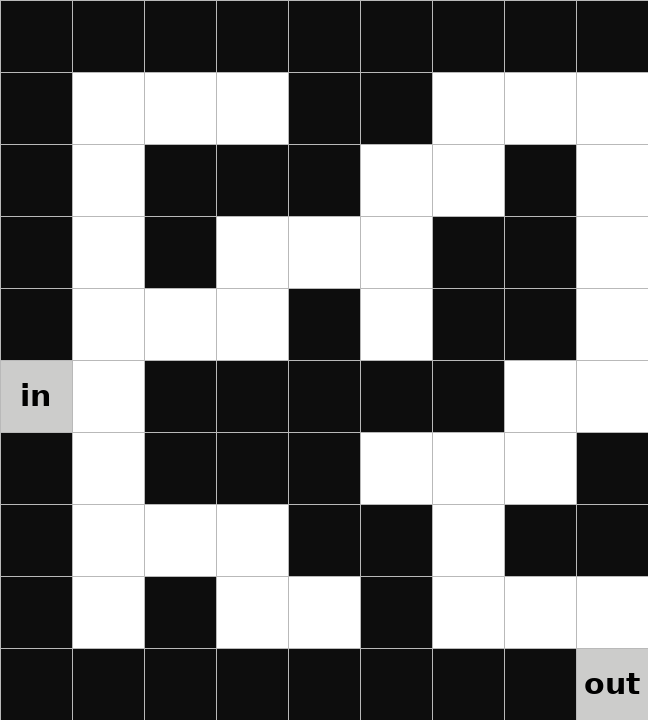
\includegraphics[width=0.42\textwidth]{figures/fig91_grid.png}

\medskip
\noindent\textbf{图 9.1\quad 一个小迷宫的例子，宝藏（出口）位于边缘}
\end{center}

但宝藏不一定非得在边缘上。图 9.2 展示了一个更大的迷宫，宝藏位于内部。

因为能看到迷宫的预览感觉很好，我们决定把自己的迷宫编码为图像。图像是表示二维（2D）网格的便捷方式，因为它有固定的大小。我们可以用颜色值编码某个网格元素是墙、路、入口还是宝藏。在前面的例子里，墙涂成黑色，路涂成白色。

% SOURCE_PDF_PAGE: 131
\begin{center}
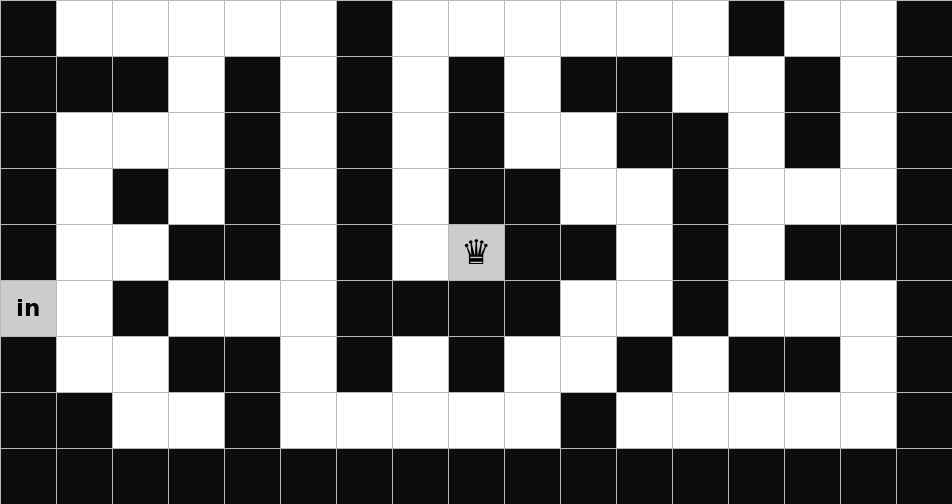
\includegraphics[width=0.60\textwidth]{figures/fig92_grid.png}

\medskip
\noindent\textbf{图 9.2\quad 宝藏位于内部的一个迷宫示例}
\end{center}

因为能看到迷宫的预览感觉很好，我们决定把自己的迷宫编码为图像。图像是表示二维网格的便捷方式，因为它有固定的大小。我们可以用颜色值编码某个网格元素是墙、路、入口还是宝藏。在前面的例子里，墙涂成黑色，路涂成白色。

\subsection{什么是图像？}

在计算机科学中，大多数 2D 图像属于两类之一：矢量图像或位图图像。矢量图像类似于数学实体——无论放大多少倍，线都没有粗细，点在屏幕上也不会显得更大，等等。可缩放矢量图形（SVG）是常见的矢量图像格式。

另一方面，位图图像（bitmap image），也称光栅图像（raster image），包含一个由图片元素组成的 2D 网格。这些图片元素（即像素）各自带有一个颜色。放大光栅图像时，像素只是被显示得更大。光栅图像的常见
% SOURCE_PDF_PAGE: 132
格式有便携式网络图形（PNG）和联合图像专家组（JPEG）。JPEG 图像提供有损压缩，这通常意味着存储信息所需的字节更少——但压缩的同时也可能修改图像。像素位置编码的通常是颜色，不过有时我们也用像素表达别的东西，例如热力图或密度（MRI 就是用图像来表示内部组织的），或者用于调色板——每种颜色都有特定含义（比如一幅世界地图，每个国家用不同颜色表示）。

因为我们想编码一个 2D 网格，光栅图像格式看起来完全够用。JPEG 的有损压缩可能导致像素颜色被改变，而我们需要精确的值来表示墙、路、入口和宝藏。因此，我们决定把图像编码为 PNG。

当然，Go 有一个用于图像操作的包，还有一个支持大多数常见图像格式的包：

\begin{shellcode}[]
> go doc image
package image // import "image"
[...]
type Image interface{ ... }
    func Decode(r io.Reader) (Image, string, error)
type Point struct{ ... }
type RGBA struct{ ... }
    func NewRGBA(r Rectangle) *RGBA
> go doc image.Point
type Point struct {
    X, Y int
}
    A Point is an X, Y coordinate pair. The axes increase right and down.
\end{shellcode}

我们在 \texttt{image} 包里看到的类型之一是 RGBAImage。它提供对 \texttt{RGBAAt(x, y)} 方法的访问，

% SOURCE_PDF_PAGE: 133
它让我们能取回图像中给定位置像素的颜色。

\subsection{迷宫的约束}

记住我们对求解器初始版本的约束：

\begin{itemize}
  \item 迷宫不会回环到自身。从入口到迷宫中任何一点都恰好只有一条路径。
  \item 生成的图像应当是使用 RGBA 颜色模型的 PNG 图像。
\end{itemize}

编写迷宫生成器时，还可以对从入口到宝藏的路径长度加一条复杂度约束，避免一眼看穿的答案。比如在我们的实现里，这条路径——也就是解——的长度必须至少是图像的高度加宽度。我们决定使用下列颜色，但你尽可以更有艺术气息、对色盲更友好：

\begin{itemize}
  \item 入口——暗色调（深蓝）
  \item 宝藏——亮色调（粉色）
  \item 墙——黑色
  \item 路——白色
\end{itemize}

现在我们有了生成的迷宫。开始解谜吧！

\section{迷宫求解器}

为了解迷宫，我们先打开生成的迷宫图像，然后探索可能的路径，同时把它们记录下来。到最后，我们会得到
% SOURCE_PDF_PAGE: 134
第一个凑合能用的版本（可能有点脏，但至少能跑），在找到宝藏时结束。

\subsection{准备工作}

跟往常一样，先建好模块并在根目录创建 \texttt{main.go}。因为这个项目是个简单的命令行工具，我们可以把 \texttt{main.go} 放在模块根目录，其余的放进 \texttt{internal} 文件夹。解迷宫的第一步是打开它。

\subsection{加载迷宫图像}

如前所述，我们希望输入 PNG 作为参数传给工具，同时传输出路径：

\begin{shellcode}[]
> maze-solver maze_10x10.png solution.png
\end{shellcode}

这意味着我们的 \texttt{main()} 要做的第一件事就是读这两个参数。

% SOURCE_PDF_PAGE: 135
\begin{gocode}[title={代码清单 9.1 \texttt{main.go}：读取参数}]
package main

import (
    "fmt"
    "log"
    "os"
)

func main() {
    if len(os.Args) != 3 { #1
        usage()
    }
    inputFile := os.Args[1] #2
    outputFile := os.Args[2]
    log.Printf("Solving maze %q and saving it as %q", inputFile, outputFile)
}

// usage displays the usage of the binary and exits the program.
func usage() {
    _, _ = fmt.Fprintln(os.Stderr, "Usage: maze_solver input.png output.png")
    os.Exit(1) #3
}

#1 Checks the number of arguments
#2 The name of the program is found at index 0 before the arguments.
#3 Exits the program with error code 1
\end{gocode}

\begin{codeannotations}
\item 检查参数数量
\item 程序名在参数之前的索引 0 处
\item 以错误码 1 退出程序
\end{codeannotations}

你已经可以运行它并检验各种场景了。接着我们打开包含迷宫的第一幅图像。此时可能发生的错误包括：根本没有文件，或图像不是 PNG。每种情况下，我们都要打印一条明确的错误。

这个操作可以用一句话概括，所以理所当然地把它放进一个函数。它接收字符串，返回 \texttt{*image.RGBA} 类型的图像。我们想要指针，因为最终我们要在写出通往宝藏的路径时修改图像。把这个函数写进一个新文件，它将包含文件 I/O 操作：

\begin{gocode}[]
func openMaze(imagePath string) (*image.RGBA, error)
\end{gocode}

就称新函数为 \texttt{openMaze} 吧。它将检查文件是否存在、打开它——别忘了 \texttt{defer} 对 \texttt{Close} 的调用——
% SOURCE_PDF_PAGE: 136
然后解码 PNG。最后一步通过调用 \texttt{image/png} 包的 \texttt{Decode} 完成，它接收一个 \texttt{io.Reader}，返回一个接口 \texttt{image.Image}。

然而不巧的是，\texttt{image.Image} 接口只提供一个访问像素值的方法——\texttt{At(x, y)}——它返回第 x 列与第 y 行交汇处像素的 \texttt{color.Color}。从普通 \texttt{image.Image} 的 \texttt{At} 返回的 \texttt{color.Color} 需要转换到 RGBA 颜色模型才可用。与其每次访问像素值都要调用 \texttt{At(x, y).RGBA()}，不如使用 \texttt{image.RGBA}——一个提供了非常方便的 \texttt{RGBAAt(x, y)} 方法的类型。为此，我们直接尝试把从文件解码出的 \texttt{image.Image} 类型断言为 \texttt{image.RGBA} 变量。

Go 提供了 \texttt{image.RGBA}，却不提供 \texttt{image.RGB}。因此本章把 RGBA 图像当作讨论对象会更简单，即便我们选择的颜色都是 100\% 不透明的。在 \texttt{main.go} 旁边创建一个名为 \texttt{imagefile.go} 的文件。

% SOURCE_PDF_PAGE: 137
\begin{gocode}[title={代码清单 9.2 \texttt{imagefile.go}：打开迷宫图像}]
package main

import (
    "fmt"
    "image"
    "image/png"
    "os"
)

// openMaze opens a RGBA png image from a path.
func openMaze(imagePath string) (*image.RGBA, error) {  #1
    f, err := os.Open(imagePath) #2
    if err != nil {
        return nil, fmt.Errorf("unable to open image %s: %w", imagePath, err)
    }
    defer f.Close()
    img, err := png.Decode(f) #3
    if err != nil {
        return nil, fmt.Errorf("unable to load input image from %s: %w",
            imagePath, err)
    }
    rgbaImage, ok := img.(*image.RGBA) #4
    if !ok {
        return nil, fmt.Errorf(
            "expected RGBA image, got %T", img) #5
    }
    return rgbaImage, nil
}

#1 Checks that the file exists
#2 Opens the file
#3 Tries decoding as a PNG
#4 Type asserts to *image.RGBA
#5 %T prints the type of a variable.
\end{gocode}

\begin{codeannotations}
\item 检查文件存在
\item 打开文件
\item 尝试按 PNG 解码
\item 类型断言为 \texttt{*image.RGBA}
\item \texttt{\%T} 打印变量的类型
\end{codeannotations}

图像到手了。别忘了在 main 里调用这个函数、妥善处理错误，并手动测试不同场景下的表现。

前面的代码里有两个错误场景很容易自动化测试：无法打开文件和无法加载 PNG 图像。要测试函数无法把它类型断言为 RGBA 图像，需要一幅不是按 RGBA 编码的 PNG 图像。我们在仓库的 \url{https://mng.bz/KGJX} 提供了这样一幅图。你应当会看到类似这样的输出：

% SOURCE_PDF_PAGE: 138
\begin{shellcode}[]
> go run . mazes/rgb.png solution.png
2023/10/16 18:26:28 INFO Solving maze "mazes/rgb.png" and saving it as
"solution.png"
ERROR: expected RGBA image, got *image.Paletted
exit status 1
\end{shellcode}

最后，还要处理``我们能检测到的文件打不开''时的 \texttt{os.Open} 错误。这种情况相当罕见——在 Unix 上，它要求你对某个目录有执行权限、却对该目录中的文件没有读权限。尽管如此，它可能发生，而知道它发生了会让我们很高兴。写个测试，然后我们就可以搭建求解部分了。

\subsection{加入求解器}

解迷宫将由一个专门的对象完成，它带有一个 \texttt{Solve()} 方法，并且可以通过传入图像来构造。为什么？这个对象将来能够持有各种设置，比如路径、墙、入口、宝藏和解（从入口到宝藏的路径）的颜色。你很快会看到，它还将持有 goroutine 之间通信的通道，以及最终的解。现在，先保持简单。

\subsubsection*{求解器结构}

Solver 是这个工具的心脏，值得住在专门的包里：\texttt{internal/solver}。记住——internal 里的包不能被你的模块之外的任何人使用。在 \texttt{internal/solver} 包中创建一个 \texttt{solver.go} 文件。

% SOURCE_PDF_PAGE: 139
\begin{gocode}[title={代码清单 9.3 \texttt{solver.go}：\texttt{Solver} 结构}]
package solver

import "image"

// Solver is capable of finding the path from the entrance to the treasure.
// The maze has to be a RGBA image.
type Solver struct {
    maze *image.RGBA
}
\end{gocode}

在继续之前，先定义这个对象的 API。它需要解迷宫并写出解的图像，如下一个清单所示。两个操作，因此是两个导出的方法。

\begin{gocode}[title={代码清单 9.4 \texttt{solver.go}：\texttt{Solve} API}]
// Solve finds the path from the entrance to the treasure.
func (s *Solver) Solve() error {
    return nil
}
\end{gocode}

\texttt{SaveSolution} 方法住在 \texttt{imagefile.go} 里，因为它属于图像操作的范畴。代码见下面的清单。

\begin{gocode}[title={代码清单 9.5 \texttt{imagefile.go}：保存解的 API}]
// SaveSolution saves the image as a PNG file
// with the solution path highlighted.
func (s *Solver) SaveSolution(outputPath string) error {
    return nil
}
\end{gocode}

\subsubsection*{NEW 函数}

实际上，我们的实现与 \texttt{image} 包高度绑定。为什么不把打开 PNG 图像这件事委托给一个 \texttt{New} 函数呢？反正我们迟早需要它。

把包含 \texttt{openImage} 函数的 \texttt{imagefile.go} 文件连同它的测试一起移到 solver 包，然后在一个叫 \texttt{New} 的新函数里调用 \texttt{openImage}。别忘了
% SOURCE_PDF_PAGE: 140
把 main 函数中先前对 \texttt{openImage} 的调用替换为对 \texttt{solver.New} 的调用。它接收路径作为参数，返回一个指向 Solver 的指针和一个错误，如下面的清单所示。注意，在一个文件里，我们倾向于把 \texttt{New} 函数和其他此类构造函数写在结构体定义之后。

\begin{gocode}[title={代码清单 9.6 \texttt{solver.go}：新建 \texttt{Solver}}]
// New builds a Solver by taking the path to the PNG maze, encoded in RGBA.
func New(imagePath string) (*Solver, error) {
    img, err := openMaze(imagePath)
    if err != nil {
        return nil, fmt.Errorf("cannot open maze image: %w", err)
    }
    return &Solver{maze: img}, nil
}
\end{gocode}

你现在的文件树应当像这样：

\begin{shellcode}[]
> tree
.
├── go.mod
├── internal
│   └── solver
│       ├── imagefile.go
│       └── solver.go
└── main.go
\end{shellcode}

此时，你甚至可以完成 main 函数的编写：按正确顺序构建 Solver 并调用其公开 API。用你喜欢的方式处理各种错误，但别忘了：命令行界面（CLI）工具出错时应当通过 \texttt{os.Exit(1)} 返回状态码 1。有任何疑问，请看 \url{https://mng.bz/9Yxj} 文件夹中的代码。

跑一跑你写的测试，提交，喝杯茶。下一节是本项目的心脏。

% SOURCE_PDF_PAGE: 141
\section{探索去也！}

上一节里，我们把迷宫图像加载进了内存。下一个目标是找到从入口到宝藏的路径，但首先得找到入口。

\subsection{寻找入口}

第一步相当直白，不过当然，如果一路上没有可学的东西，我们也不会写这本书了。把图像加载进内存并不意味着就能立刻解迷宫。首先，我们得知道怎么探索它。

\subsubsection*{调色板}

为了编码信息，迷宫生成器用像素在特定位置存储特定值。在我们的迷宫里，这些值表示墙、路、入口和宝藏。我们想把像素的颜色与这些特定值进行比较。RGBA 颜色在 \texttt{image/color} 包中以结构体表示，而结构体不能是常量，这意味着我们表示路、墙、入口和宝藏的参照色不能是常量。那我们怎么引用它们？有几个方案。

一种办法是把颜色声明为 solver 包里的全局变量。嗯，我们不喜欢全局变量：它们可能被误改、逃过所有测试的火眼金睛，然后整个行为变得完全无法解释。作为第一步它还行，但我们不希望它在生产环境里出现。

一个有意思的替代方案是创建一个调色板（palette）结构来持有所有不同的值。你可以在迷宫求解器运行时从
% SOURCE_PDF_PAGE: 142
配置文件加载调色板，但这超出了本章的范围。只要 main 包不需要修改这些值，我们就无需暴露这个结构。在 \texttt{internal/solver} 包里创建一个名为 \texttt{palette.go} 的文件。

\begin{gocode}[title={代码清单 9.7 \texttt{palette.go}：声明颜色列表}]
// palette contains the colours of the different types of pixels in our maze.
type palette struct {
    wall        color.RGBA
    path        color.RGBA #1
    entrance    color.RGBA #2
    treasure    color.RGBA
    solution    color.RGBA #3
}

#1 The color of the possible paths
#2 The pixel you're looking for
#3 Displays the solution
\end{gocode}

\begin{codeannotations}
\item 可能路径的颜色
\item 你要找的像素
\item 显示解
\end{codeannotations}

一个填好我们所选值的调色板结构可以由 \texttt{defaultPalette()} 函数返回，如代码清单 9.8 所示。相比全局变量的优势是：函数返回的值谁也改不了。遗憾的是，每次需要它都会创建一个新结构体，分配出需要垃圾回收的宝贵内存。一旦开始探索更大的迷宫，这就可能变得昂贵。

% SOURCE_PDF_PAGE: 143
\begin{gocode}[title={代码清单 9.8 \texttt{palette.go}：默认颜色函数}]
// defaultPalette returns the colour palette of our maze.
func defaultPalette() palette {
    return palette{
        wall:     color.RGBA{
            R: 0,   G: 0,   B: 0,   A: 255},  #1
        path:     color.RGBA{
            R: 255, G: 255, B: 255, A: 255}, #2
        entrance: color.RGBA{
            R: 0,   G: 191, B: 255, A: 255}, #3
        treasure: color.RGBA{
            R: 255, G: 0,   B: 128, A: 255}, #4
        solution: color.RGBA{
            R: 225, G: 140, B: 0,   A: 255}, #5
    }
}

#1 Black
#2 White
#3 Deep blue
#4 Pink
#5 Orange
\end{gocode}

\begin{codeannotations}
\item 黑色
\item 白色
\item 深蓝
\item 粉色
\item 橙色
\end{codeannotations}

我们实际做的，是把这些值作为求解这幅图像的设置保存在 Solver 结构里（见代码清单 9.9）。这很合理，因为另一个求解器面对另一幅图时，可以使用另一套颜色。

\begin{gocode}[title={代码清单 9.9 \texttt{solver.go}：带调色板的 \texttt{Solver}}]
type Solver struct {
    maze     *image.RGBA
    palette   palette
}
\end{gocode}

目前，你只需在 solver 包的 \texttt{New} 函数里用刚定义的 \texttt{defaultPalette()} 把这些颜色设为默认值。现在，循着指示牌去找入口吧。

\subsubsection*{像素定义}

我们将通过探索像素来穿越迷宫，像素由它们在 2D 图像上的坐标标识。既然要在这些 2D 网格中导航，就用 Go 提供的 \texttt{image.Point} 吧：

% SOURCE_PDF_PAGE: 144
\begin{gocode}[]
type Point struct {
    X, Y int
}
\end{gocode}

关于像素，有一点可以轻易预见：我们需要找到它的开放邻居——与它正交相连、带有路颜色的像素。如果像素能告诉我们自己邻居的坐标，事情会容易得多。由于迷宫的实现方式，我们不想包含对角相邻的邻居。在 \texttt{internal/solver} 包中创建一个名为 \texttt{neighbours.go} 的文件，编写 \texttt{neighbours} 函数。

\begin{gocode}[title={代码清单 9.10 \texttt{neighbours.go}：像素的坐标}]
package solver

import "image"

// neighbours returns an array of the 4 neighbours of a pixel.
// Some returned positions may be outside the image.
func neighbours(p image.Point) [4]image.Point {
    return [...]image.Point{
        {p.X, p.Y + 1}, #1
        {p.X, p.Y - 1}, #2
        {p.X + 1, p.Y}, #3
        {p.X - 1, p.Y}, #4
    }
}

#1 One pixel down
#2 One pixel up
#3 One pixel to the right
#4 One pixel to the left
\end{gocode}

\begin{codeannotations}
\item 下一个像素
\item 上一个像素
\item 右侧一个像素
\item 左侧一个像素
\end{codeannotations}

\begin{infobox}{注意}
这个函数返回一个数组。写成 \texttt{[...]image.Point}，表示让编译器推断数组长度；在这里，它等价于 \texttt{[4]image.Point}。使用数组算是一项小优化：它更有可能分配在栈上，而不是堆上。
\end{infobox}

这个函数没有任何东西保证邻居在图像之内。比如，位于 (0, 0) 的左上角像素有两个邻居在图像之外。我们可以
% SOURCE_PDF_PAGE: 145
在这里加一道安全网，或者规定图像的边缘一律不予探索。

另一种思路是想想我们会怎么使用这些邻居。稍后在代码里，我们要检查它们代表迷宫中可探索的一段、一堵墙、宝藏，还是我们编码的其他信息。为此，必须查看每个邻居的 \texttt{RGBAAt(position)} 返回值。查一下它的实现就会发现：当位置在图像之外时，\texttt{RGBAAt} 返回零值。这意味着让 \texttt{neighbours} 返回超出图像边界的点是安全的。

API 不保证的另一件事是邻居的顺序。我们可以从上方开始顺时针排列，也可以狂野一点直接打乱。这意味着编写测试正是使用 \url{https://github.com/stretchr/testify} 框架及其 \texttt{assert.ElementsMatch} 函数的绝佳时机。

\subsubsection*{找到入口的像素}

回到 \texttt{solver.go} 文件，创建函数 \texttt{findEntrance}。我们必须扫描整幅图像，找到一个具有入口颜色的像素。要检查每个像素的值，图像处理中的一个常见做法是按行优先顺序（row-major order）使用两层嵌套循环：外层循环遍历图像的各行，内层循环遍历行中的各列。这类似于某些语言（如英语或提菲纳格字母）书写文本的方式：从最左写到最右，然后换行，再从最左开始。

之所以是这种特定模式，是因为图像格式往往以扫描线（scanline）格式存储像素值，
% SOURCE_PDF_PAGE: 146
图像中水平相邻的像素被存储在相邻的内存位置。想到大多数图像格式的开发者都以英语为母语，这一点就好理解了。

大多数时候，我们迷宫的第一个像素位于 (0, 0)——左上角。但如果我们看的是图像的一个子区域，我们的``左上角''可能在别的位置。这里可以通过 \texttt{image.RGBA} 类型的 \texttt{Bounds()} 方法访问迷宫的边界。它返回定义图像包围盒的两个点：\texttt{Min} 和 \texttt{Max} 字段。

\begin{gocode}[title={代码清单 9.11 \texttt{solver.go}：寻找入口}]
// findEntrance returns the position of the maze entrance on the image.
func (s *Solver) findEntrance() (image.Point, error) {
    for row := s.maze.Bounds().Min.Y; row < s.maze.Bounds().Max.Y; row++ {
        for col := s.maze.Bounds().Min.X; col < s.maze.Bounds().Max.X; col++
    {
            if s.maze.RGBAAt(col, row) == s.palette.entrance {
                return image.Point{X: col, Y: row}, nil #1
            }
        }
    }
    return image.Point{}, fmt.Errorf("entrance position not found")
}

#1 Returns as soon as we find an entrance
\end{gocode}

\begin{codeannotations}
\item 一找到入口就返回
\end{codeannotations}

回到 \texttt{Solve} 方法，我们可以调用它来确定起点，如下面的清单所示。

\begin{gocode}[title={代码清单 9.12 \texttt{solver.go}：在 \texttt{Solve} 中调用 \texttt{findEntrance}}]
// Solve finds the path from the entrance to the treasure.
func (s *Solver) Solve() error {
    entrance, err := s.findEntrance()
    if err != nil {
        return fmt.Errorf("unable to find entrance: %w", err)
    }
    log.Printf("starting at %v", entrance))
    return nil
}
\end{gocode}

% SOURCE_PDF_PAGE: 147
如果没有入口怎么办？确保在测试中覆盖各种情形。也许我们希望迷宫只有一个入口。如果你写测试时遇到困难，可以在 \url{https://mng.bz/jpMa} 的文件里找到我们的测试用例，所有场景使用的迷宫图像都放在本书仓库的 \texttt{internal/solver/testdata} 下（\url{https://mng.bz/GeMv}）。图 9.3 展示了一个已识别出入口的迷宫。

\begin{center}
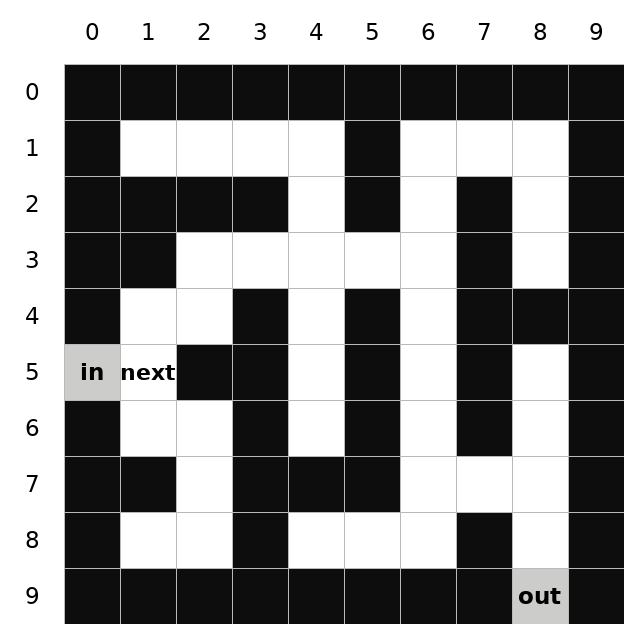
\includegraphics[width=0.44\textwidth]{figures/fig93_grid.png}

\medskip
\noindent\textbf{图 9.3\quad 标出入口和下一个像素的迷宫}
\end{center}

我们已经从入口踏进迷宫并探索了一个像素。现在需要探索下一个（些）像素，才能抵达宝藏。

\subsection{传达新的可行路径}

解迷宫的优化算法很多，但大多采用迭代式的方法——在每个转角左转、前往既离入口最近又未探索过的位置，等等。
% SOURCE_PDF_PAGE: 148
每当遇到一个岔路口，都必须做出决策：先左、再右、然后直行？本章我们用一个问句回答这个问题：为什么不同时试所有方向？这就需要并行编程，在 Go 中用 goroutine 实现。每次发现路径分岔，我们会想沿着其中一个可能方向继续，并为其他方向启动 goroutine。使用 goroutine 意味着我们可以把其他方向的探索委托出去，专注走完当前分支，直到抵达宝藏或死胡同。

使用 goroutine 可以提升性能——让找到解的速度更快——但这并非保证。启动 goroutine 需要时间，与它们通信还会增加额外开销。通常，对非常快的任务来说 goroutine 并非必要。在我们的例子里，每个 goroutine 的作用范围都无法确定：我们不知道它何时结束，那不妨给它一个机会。

可以确定的是，使用 goroutine 会增加 CPU 的使用。在图 9.4 中，我们要寻找宝藏（$\mu$）。goroutine 代达罗斯（$\delta$）从 A5 出发，然后到 B5，需要分岔。第二个 goroutine 忒修斯（$\theta$）从 B6 接手，而 $\delta$ 继续走向 B4、C4 等等。只要迷宫里没有环，代达罗斯和忒修斯在探索迷宫时就不会相遇，这意味着代达罗斯完全不需要知道忒修斯的存在。

% 图 9.4：代达罗斯与忒修斯的并发探索（依原书重绘）
\begin{center}
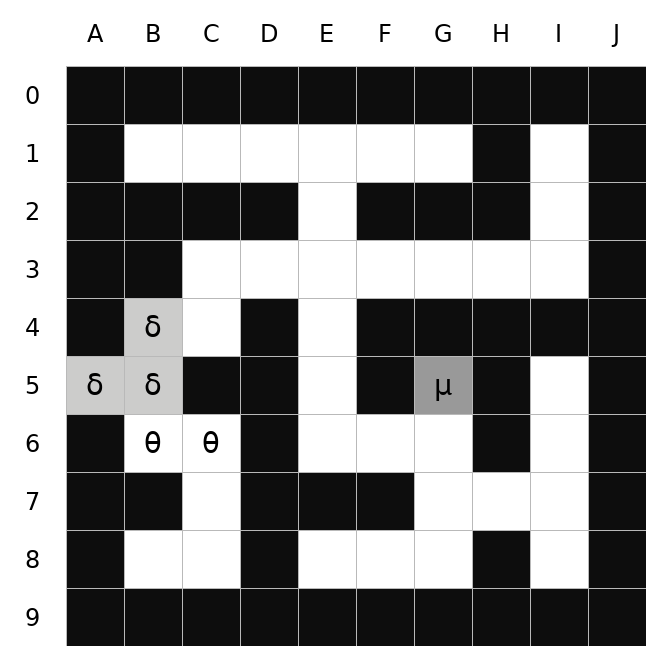
\includegraphics[width=0.44\textwidth]{figures/fig94_grid.png}

\medskip
\noindent\textbf{图 9.4\quad 由不同 goroutine 进行的探索}
\end{center}

% SOURCE_PDF_PAGE: 149
从那里开始，两个 goroutine 继续探索，不断启动新的探索者。抵达宝藏的探索过程可能看起来像图 9.5（每个 goroutine 探索过的路径用不同的希腊字母表示）。

% 图 9.5：一次可能的事件序列的探索（依原书重绘）
\begin{center}
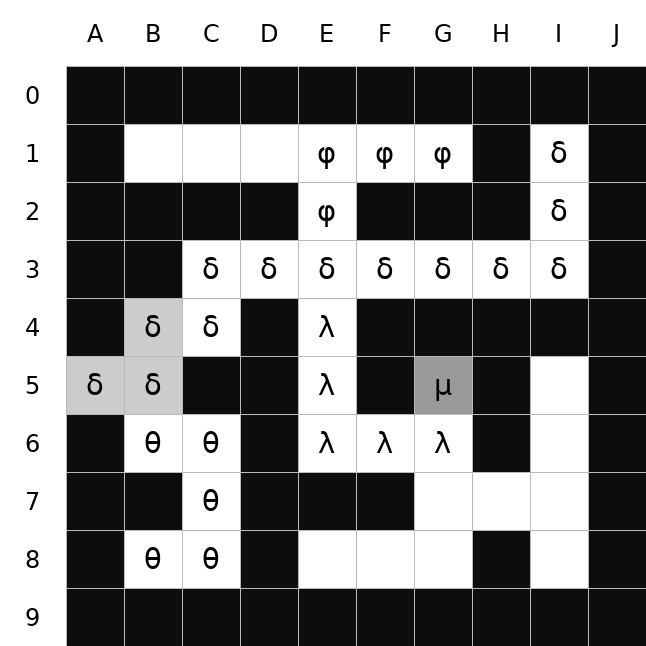
\includegraphics[width=0.44\textwidth]{figures/fig95_grid.png}

\medskip
\noindent\textbf{图 9.5\quad 表示一次可能的事件序列的探索}
\end{center}

\begin{infobox}{注意}
goroutine 之间的通信是通道的用途所在。
\end{infobox}

找到入口的位置后，我们的 \texttt{Solve} 函数负责从那里开始，发起对迷宫的探索。一旦有新路径要探索，我们就希望求解器开始对那条分支的探索。每个探索者负责通过通道向求解器通报新分支，% SOURCE_PDF_PAGE: 150
求解器则监听这些通知。由此我们明白：需要给求解器添加两个新方法——第一个探索一条路径，不妨叫 \texttt{explore}；第二个负责监听各条分支，就叫它 \texttt{listenToBranches} 吧。我们的求解器通过向通道发送一条消息来发起对迷宫的探索，而 \texttt{listenToBranches} 方法正在监听这个通道。

% SOURCE_PDF_PAGE: 151
\texttt{listenToBranches} 函数读出第一条消息，为一个从 A5 出发的路径创建 goroutine——就是我们叫作代达罗斯（$\delta$）的那个。图 9.6 展示了以下事件的示意图。代达罗斯查看 A5 的邻居：只有 B5 合格。这个 goroutine 把 B5 纳入自己已探索的路径，再查看 B5 的邻居，发现 B4 和 B6 是值得探索的候选。我们这位探索者 goroutine——代达罗斯——把通往 B6 的路径发送到通道，继续探索 B4、C4 等等。通道的监听者读出代达罗斯发来的消息，启动一个新的 goroutine——忒修斯（$\theta$）——它接着走向 C6、C7 等等，直到撞见死胡同而结束。与此同时，代达罗斯已抵达 E3，面临三条新的探索路径。它（随机地）选择继续走自己的路（D3、E3、C3），把通向 E2 和 E4 的路径发送到通道，监听者又启动了两个新 goroutine，$\lambda$ 和 $\varphi$。

当然，在这个场景里，请对文中的语法时态持保留态度——因为取决于你的架构和 CPU 随机决定的重新调度，未来、现在与过去可能每次运行都不一样。动手实现它有助于我们更好地理解这些细节。

% SOURCE_PDF_PAGE: 152
% 图 9.6：Solve 中事件的先后顺序（依原书重绘的时序图）
\begin{center}
\begin{tikzpicture}[
  x=1cm, y=1cm,
  part/.style={draw=PocketTealDark, thick, rounded corners=1.2mm, fill=PocketMist,
               font=\ttfamily\scriptsize, inner sep=3pt, minimum height=5.2mm},
  msg/.style={-{Stealth[length=2.2mm]}, thick},
  lbl/.style={font=\ttfamily\tiny, above=1.3pt, midway, fill=white, inner sep=0.7pt},
  lifeline/.style={dashed, black!55, thick},
  act/.style={draw=black!70, fill=white, thick},
]
% Six participants only: the E4 branch is intentionally launched off-chart,
% matching the source sequence diagram rather than inventing a seventh lifeline.
\def\axS{-0.35} % Solve
\def\axL{2.10}  % listenToBranches
\def\axE{4.35}  % explore
\def\axD{6.10}  % for loop delta
\def\axT{8.05}  % for loop theta
\def\axF{10.05} % for loop varphi

% lifelines
\foreach \x in {\axS,\axL,\axE,\axD,\axT,\axF}
  {\draw[lifeline] (\x,-0.50) -- (\x,-13.05);}

% participant boxes (top and bottom)
\foreach \x/\name in {\axS/{Solve}, \axL/{listenToBranches}, \axE/{explore},
                      \axD/{for~loop $\delta$}, \axT/{for~loop $\theta$}, \axF/{for~loop $\varphi$}}
  {\node[part] at (\x,0) {\name}; \node[part] at (\x,-13.45) {\name};}

% activations
\filldraw[act] (\axL-0.08,-0.62) rectangle (\axL+0.08,-12.72);
\filldraw[act] (\axE-0.08,-1.08) rectangle (\axE+0.08,-1.78);
\filldraw[act] (\axD-0.08,-1.68) rectangle (\axD+0.08,-12.82);
\filldraw[act] (\axT-0.08,-3.98) rectangle (\axT+0.08,-11.92);
\filldraw[act] (\axF-0.08,-7.92) rectangle (\axF+0.08,-12.02);

% Solve starts the listener.
\draw[msg] (\axS,-0.62) -- (\axL,-0.62);

% Listener asks explore to begin at A5, then explore launches Daedalus (delta).
\draw[msg] (\axL,-1.15) -- node[lbl]{go $\delta$ on A5} (\axE,-1.15);
\draw[msg] (\axE,-1.68) -- (\axD,-1.68);

% B5 and B4 are explored by delta (not by the explore dispatcher).
\node[font=\ttfamily\scriptsize,anchor=south west] at (\axD+0.18,-2.05) {B5};
\draw[thick] (\axD+0.08,-2.02) -- (\axD+0.78,-2.02) -- (\axD+0.78,-2.34);
\draw[msg] (\axD+0.78,-2.34) -- (\axD+0.08,-2.34);
\node[font=\ttfamily\scriptsize,anchor=south west] at (\axD+0.18,-2.66) {B4};
\draw[thick] (\axD+0.08,-2.63) -- (\axD+0.78,-2.63) -- (\axD+0.78,-2.95);
\draw[msg] (\axD+0.78,-2.95) -- (\axD+0.08,-2.95);

% Delta publishes the B6 branch; the listener starts Theseus (theta).
\draw[msg] (\axD,-3.38) -- node[lbl]{A5, B5, B6} (\axL,-3.38);
\draw[msg] (\axL,-3.98) -- node[lbl]{go $\theta$ on A5, B5, B6} (\axT,-3.98);

% Concurrent exploration on delta and theta.
\node[font=\ttfamily\scriptsize,anchor=south west] at (\axD+0.18,-4.48) {C4, \ldots, E3};
\draw[thick] (\axD+0.08,-4.45) -- (\axD+0.98,-4.45) -- (\axD+0.98,-4.77);
\draw[msg] (\axD+0.98,-4.77) -- (\axD+0.08,-4.77);

\node[font=\ttfamily\scriptsize,anchor=south west] at (\axT+0.18,-4.72) {C6};
\draw[thick] (\axT+0.08,-4.69) -- (\axT+0.78,-4.69) -- (\axT+0.78,-5.01);
\draw[msg] (\axT+0.78,-5.01) -- (\axT+0.08,-5.01);
\node[font=\ttfamily\scriptsize,anchor=south west] at (\axT+0.18,-5.48) {C7};
\draw[thick] (\axT+0.08,-5.45) -- (\axT+0.78,-5.45) -- (\axT+0.78,-5.77);
\draw[msg] (\axT+0.78,-5.77) -- (\axT+0.08,-5.77);
\node[font=\ttfamily\scriptsize,anchor=south west] at (\axT+0.18,-6.24) {C8};
\draw[thick] (\axT+0.08,-6.21) -- (\axT+0.78,-6.21) -- (\axT+0.78,-6.53);
\draw[msg] (\axT+0.78,-6.53) -- (\axT+0.08,-6.53);

% At E3 delta publishes the E2 and E4 branches.
\draw[msg] (\axD,-6.82) -- node[lbl]{A5, B5, \ldots, E3, E2} (\axL,-6.82);
\draw[msg] (\axD,-7.38) -- node[lbl]{A5, B5, \ldots, E3, E4} (\axL,-7.38);

% The listener starts varphi on E2; the E4 branch is another goroutine outside this chart.
\draw[msg] (\axL,-7.95) -- node[lbl]{go $\varphi$ on A5, B5, \ldots, E3, E2} (\axF,-7.95);
\draw[msg,dashed] (\axL,-8.50) -- node[lbl]{go A5, B5, \ldots, E3, E4} (11.28,-8.50);

% Later events on the three visible worker goroutines.
\node[font=\ttfamily\scriptsize,anchor=south west] at (\axD+0.18,-9.13) {F3};
\draw[thick] (\axD+0.08,-9.10) -- (\axD+0.78,-9.10) -- (\axD+0.78,-9.42);
\draw[msg] (\axD+0.78,-9.42) -- (\axD+0.08,-9.42);

\node[font=\ttfamily\scriptsize,anchor=south west] at (\axT+0.18,-9.28) {B8};
\draw[thick] (\axT+0.08,-9.25) -- (\axT+0.78,-9.25) -- (\axT+0.78,-9.57);
\draw[msg] (\axT+0.78,-9.57) -- (\axT+0.08,-9.57);

\node[font=\ttfamily\scriptsize,anchor=south west] at (\axF+0.18,-9.43) {E1};
\draw[thick] (\axF+0.08,-9.40) -- (\axF+0.78,-9.40) -- (\axF+0.78,-9.72);
\draw[msg] (\axF+0.78,-9.72) -- (\axF+0.08,-9.72);

% Varphi publishes the branch through D1 back to the listener.
\draw[msg] (\axF,-10.25) -- node[lbl]{A5, \ldots, E1, D1} (\axL,-10.25);

\node[font=\ttfamily\scriptsize,anchor=south west] at (\axD+0.18,-10.92) {G3};
\draw[thick] (\axD+0.08,-10.89) -- (\axD+0.78,-10.89) -- (\axD+0.78,-11.21);
\draw[msg] (\axD+0.78,-11.21) -- (\axD+0.08,-11.21);

\node[font=\ttfamily\scriptsize,anchor=south west] at (\axT+0.18,-10.92) {Dead end.};
\draw[thick] (\axT+0.08,-10.89) -- (\axT+1.02,-10.89) -- (\axT+1.02,-11.21);
\draw[msg] (\axT+1.02,-11.21) -- (\axT+0.08,-11.21);
\draw[thick,black] (\axT-0.22,-11.52) -- (\axT+0.22,-11.78)
                   (\axT-0.22,-11.78) -- (\axT+0.22,-11.52);

\node[font=\ttfamily\scriptsize,anchor=south west] at (\axF+0.18,-11.08) {F1};
\draw[thick] (\axF+0.08,-11.05) -- (\axF+0.78,-11.05) -- (\axF+0.78,-11.37);
\draw[msg] (\axF+0.78,-11.37) -- (\axF+0.08,-11.37);

% Listener returns to Solve after the winning branch is reported.
\draw[msg] (\axL,-12.55) -- (\axS,-12.55);
\end{tikzpicture}

\medskip
\noindent\textbf{图 9.6\quad \texttt{Solve} 中事件的先后顺序}
\end{center}

为了让代达罗斯启动一个自主的 goroutine，让它能够从 B6 继续探索路径，它只需把到目前为止的路径传达给忒修斯和那个抵达宝藏的 goroutine。仅此而已。它们需要知道经由已探索像素抵达此处所走的路径，我们可以把它表示为 \texttt{image.Point} 的链表，如代码清单 9.13 所示。创建 \texttt{internal/solver/path.go} 文件，加上 \texttt{path} 结构。

% SOURCE_PDF_PAGE: 153
\begin{gocode}[title={代码清单 9.13 \texttt{path.go}：用链表存储迄今为止的路径}]
package solver

import "image"

// path represents a route from the entrance of the maze up to a position.
type path struct {
    previousStep *path
    at           image.Point
}
\end{gocode}

给 Solver 加一个字段，它是一个通道，其消息是指向 \texttt{path} 的指针。

\begin{gocode}[title={代码清单 9.14 \texttt{solver.go}：给 \texttt{Solver} 结构添加通道}]
type Solver struct {
    maze           *image.RGBA
    palette        palette
    pathsToExplore chan *path #1
}

#1 A channel that carries linked lists of explored pixels
\end{gocode}

\begin{codeannotations}
\item 一个承载已探索像素链表的通道
\end{codeannotations}

这里就是 goroutine 发布新待探索路径的地方，也是 \texttt{listenToBranches} 方法监听并启动新探索 goroutine 的地方。该方法将在 9.3.4 节加入，因为常识告诉我们：只要通道还开着，就不能从一个还没写入任何东西的通道里读取。

\subsection{记录已探索的路径}

考虑到这个程序的目的是告诉我们如何从一点走到另一点，每探索一个新像素时，我们都需要知道自己是怎么到这里的。我们不能像法国童话里的小拇指（Hop-o'-My-Thumb）那样一路丢石子，但计算机的内存完全可以为我所用。

% SOURCE_PDF_PAGE: 154
\subsubsection*{每个 goroutine 的行为}

我们来写 \texttt{explore} 函数：它接收一条路径作为参数并探索它。这个函数会一直运行，直到找到死胡同或宝藏，并把它不走的分支发布到通道上。这个函数包含每个 goroutine 要做的事。

第一版里，如果找到了宝藏，我们先只打印一条消息，然后用 \texttt{return} 停止探索。这个后面再回来处理。

我们选择把这个函数放进 solver 包中一个专门的文件 \texttt{explore.go}，如代码清单 9.15 所示。这个函数足够重要，我们会经常回头调试它。

% SOURCE_PDF_PAGE: 155
\begin{gocode}[title={代码清单 9.15 \texttt{explore.go}：探索一条路径}]
package solver

import (
    "image"
    "log"
)

// explore one path and publish to the s.pathsToExplore channel
// any branch we discover that we don't take.
func (s *Solver) explore(pathToBranch *path) {
    if pathToBranch == nil {
        // This is a safety net. It should be used, but when it's needed,
        // at least it's there.
        return
    }
    pos := pathToBranch.at #1
    for {
// We know we'll have up to 3 new neighbours to explore.#2
        candidates := make([]image.Point, 0, 3)
        for _, n := range neighbours(pos) { #3
            if  pathToBranch.isPreviousStep(n){ #4
                // Let's not return to the previous position
                continue
            }
            // Look at the colour of this pixel.
            // RGBAAt returns a color.RGBA{} zero value if the pixel is
            // outside the bounds of the image.
            switch s.maze.RGBAAt(n.X, n.Y) { #5
            case s.palette.treasure:
                log.Printf("Treasure found at %v!", n)
                return
            case s.palette.path: #6
                candidates = append(candidates, n)
            }
        }
        if len(candidates) == 0 {
            log.Printf("I must have taken the wrong turn at position %v.",
                pos)
            return
        }
        // See below
    }
}

// isPreviousStep returns true if the given point is
// the previous position of the path.
func (p path) isPreviousStep(n image.Point) bool {
    return p.previousStep != nil && p.previousStep.at == n
}

#1 This is the pixel we're at.
#2 Forever until we break out or find a dead end
#3 Peeks in each direction for path pixels
% SOURCE_PDF_PAGE: 156
#4 This is where we came from.
#5 Checks the color of the neighbor
#6 This is a valid candidate.
\end{gocode}

\begin{codeannotations}
\item 这就是我们所在的像素
\item 直到 break 或找到死胡同才结束
\item 向各个方向探测路径像素
\item 这是我们来的地方
\item 检查邻居的颜色
\item 这是一个有效候选
\end{codeannotations}

注意，到目前为止，邻居只能是墙、路、入口或宝藏。入口已经被跳过，因为它是前一个像素；墙我们无能为力。这就是 switch 里只有两个 case 的原因——而且我们没有添加空的 default 分支：我们要么找到宝藏，要么找到下一个可探索的位置，别的东西都无趣。很重要的一点是：在寻找合格邻居时，我们不想原路返回、退回前一个位置。那会导致 goroutine 无休止地创建、程序崩溃。我们会在 9.6.1 节探讨阻止这种情况的方法。

然后有两种情况要考虑：要么没有下一个像素可探索——那就是死胡同；要么有下一个像素可探索，那就得向监听的 goroutine 发消息。死胡同的情形，我们打印一条日志消息来了解发生了什么，此外无事可做。我们退出循环，goroutine 结束自己的执行。

\subsubsection*{分岔}

如果确实有一个或多个待探索的像素候选，我们给自己留一个（在我们的例子里是第一个，\texttt{candidates[0]}），并把其余路径发送到通道上，如下面的清单所示。然后，我们继续把探索向前推进一步。

% SOURCE_PDF_PAGE: 157
\begin{gocode}[title={代码清单 9.16 \texttt{explore.go}：继续探索}]
for _, candidate := range candidates[1:] { #1
    branch := &path{previousStep: pathToBranch, at: candidate}
    s.pathsToExplore <- branch #2
}
pathToBranch = &path{
    previousStep: pathToBranch,
    at: candidates[0]} #3
pos = candidates[0]

#1 Ignores candidates[0]
#2 Publishes the path leading to the branch
#3 Continues exploring
\end{gocode}

\begin{codeannotations}
\item 忽略 \texttt{candidates[0]}
\item 发布通往分支的路径
\item 继续探索
\end{codeannotations}

这是个相当长的函数。我们可以通过抽取逻辑片段来重构。循环通常是个好候选，因为它们可以用一句话概括，在逻辑上是一个单元。看看我们的选项：

\begin{itemize}
  \item 抽取大无限循环的内部。这个选项要返回的变量太多：下一个位置、下一个``前一个''位置、是否退出的信号，可能还有一个错误。
  \item 抽取第一部分，即我们寻找候选的部分。这是我们选择在成功时退出的地方。可行，但不太容易。
  \item 抽取第二个 switch，即我们查看候选的部分。这种情况下，我们也会在死胡同时退出。我们可以把发布循环抽出来，但为了三行代码，代码真的会变得更容易理解吗？
\end{itemize}

先保持现状，看看写测试是不是过于复杂。常言道，因为我们想尽可能隔离逻辑，测试往往比代码本身更复杂一点，并且至少需要同样的概念，所以我们打算再稍等片刻。不过，可别养成习惯。

% SOURCE_PDF_PAGE: 158
\subsection{等待未探索的路径并启动 goroutine}

探索时，我们需要一个函数来监听通道，并为通道里的每条消息启动一个新 goroutine。它不必复杂：对通道里的每条消息，调用 \texttt{explore}，如代码清单 9.17 所示。

Go 中监听发布到通道的所有消息的关键字是 \texttt{range}，与切片或映射上的用法完全一样。对通道使用 \texttt{range} 是阻塞的，也就是说，只要 \texttt{close(s.pathsToExplore)} 没被调用，这个函数就会一直等待通道上发布的消息。

\begin{gocode}[title={代码清单 9.17 \texttt{explore.go}：监听通道}]
// listenToBranches creates a new goroutine for each branch published in
// s.pathsToExplore.
func (s *Solver) listenToBranches() {
    for p := range s.pathsToExplore {
        go s.explore(p)
    }
}
\end{gocode}

这是一个非常短的实现；它能工作，但对 goroutine 来说有个隐患。我们知道它们何时开始，却不知道何时结束。这里，我们没有追踪各个 goroutine（也没追踪它们的数量），这意味着程序可能在它们还在运行、还在占用内存和 CPU 时就结束了。在我们的代码被算作正确之前，需要先修复这一点。

但先让程序跑起来。启动探索要做的最后一件事是发布第一条消息。为了启动第一个 goroutine——我们在例子里叫它代达罗斯的那个——只需要把入口发布到通道并开始监听。

回到 \texttt{Solve} 函数。它知道入口像素的位置，我们可以把它发布出去：

% SOURCE_PDF_PAGE: 159
\begin{gocode}[]
s.pathsToExplore <- &path{previousStep: nil, at: entrance}
\end{gocode}

别忘了在那之后调用监听函数 \texttt{listenTobranches}，然后试着运行程序。有报错吗？你应当会看到。我们现在得到的是：

\begin{shellcode}[]
fatal error: all goroutines are asleep - deadlock!
goroutine 1 [chan send (nil chan)]:
learngo/09/maze/internal/solver.(*Solver).Solve(0x1400009c180)
\end{shellcode}

我们正试图对一个 nil 通道又写又读。在 \texttt{New} 函数里初始化通道，然后像下面这样再试：

\begin{gocode}[]
pathsToExplore: make(chan *path),
\end{gocode}

还是同样的问题。我们选了无缓冲通道，在读取之前向它发送消息会一直触发致命错误。

\begin{infobox}{注意}
对无缓冲通道的发送操作会阻塞发送的 goroutine，直到同一通道上发生对应的接收。此时，值被传递，两个 goroutine 才能继续。关于无缓冲通道的更多内容，请参阅 Alan A. A. Donovan 与 Brian W. Kernighan 的《The Go Programming Language》（Addison-Wesley Professional，2015）。
\end{infobox}

在开始读取之前，我们不能写无缓冲通道。作为替代，可以给通道一个单值缓冲。一个值就够了，因为写完这个值之后，我们的主 goroutine 会永远监听：

\begin{gocode}[]
pathsToExplore: make(chan *point, 1),
\end{gocode}

或者，如果我们当初建的是无缓冲通道 \texttt{make(chan *point)}，\texttt{Solve} 函数里对通道的写入也可以放进一个 goroutine 里做：

% SOURCE_PDF_PAGE: 160
\begin{gocode}[]
go func() { s.pathsToExplore <- &path{previousStep: nil, at: entrance} }()
\end{gocode}

如你所见，只要日志到处都是，缓冲大小取 1 就足以解出一个小迷宫，但程序最终仍会以死锁收场。如前所说，主 goroutine 会永远监听，即使所有子例程早已停止发布。Go 会注意到这一点，稍过片刻以死锁错误结束执行。我们需要一种办法告诉监听方法停下来。

\subsection{别听了，找到了：简短版}

当某个 goroutine 找到宝藏时，它需要把通往宝藏的路径存在某个地方，并设法告诉所有其他 goroutine 别再找了，同时告诉监听者别再听了。我们先实现一个快速版本，以便尽快看到漂亮的东西、看到它的局限，再找出更好的方案。

几页之前我们抄了个小近道，就在找到宝藏的地方。此时，我们需要把像素路径保存在 \texttt{SaveSolution} 函数能找到的地方。多数情况下，把它放进 Solver 里就足够好了，如代码清单 9.18 所示。另外，它还可以充当一个旗标，告诉各个 goroutine 宝藏已经找到、可以停止寻找了。

\begin{gocode}[title={代码清单 9.18 \texttt{solver.go}：添加解}]
type Solver struct {
    maze         *image.RGBA
    palette       palette
    pathsToExplore   chan *path
    solution *path #1
}

#1 Saves the solution
\end{gocode}

\begin{codeannotations}
\item 保存解
\end{codeannotations}

在 \texttt{explore} 函数里，给这个字段赋值只需要一行。回到那个 switch，如后面的清单所示。

% SOURCE_PDF_PAGE: 161
\begin{gocode}[title={代码清单 9.19 \texttt{explore.go}：保存解}]
case s.palette.treasure:
    s.solution = &path{previousStep: pathToBranch, at: n} #1
    log.Printf("Treasure found at %v!", n))
    return

#1 Adds the treasure to the path
\end{gocode}

\begin{codeannotations}
\item 把宝藏加进路径
\end{codeannotations}

等等——任何 goroutine 都可能写 \texttt{s.solution}，那怎么避免制造数据竞争？加一个互斥锁来保护自己吧。这个互斥锁是 Solver 结构的新字段。下面的清单展示我们在 treasure 这个 case 里如何使用它。

\begin{gocode}[title={代码清单 9.20 \texttt{explore.go}：用互斥锁保存解}]
case s.palette.treasure:
    s.mutex.Lock()
    defer s.mutex.Unlock() #1
    if s.solution == nil {
        s.solution = &path{previousStep: pathToBranch, at: n}
        log.Printf("Treasure found at %v!", n))
    }
    return

#1 It's OK to defer despite being in a loop because this case always
returns.
\end{gocode}

\begin{codeannotations}
\item 尽管处在循环里，这里 \texttt{defer} 也没问题，因为这个 case 总会返回
\end{codeannotations}

接着，为了告诉其他 goroutine 停下来，我们把这个解字段当作旗标用。诚然这不是什么好方案，但它够快。因为要在好几处检查解是否已找到，我们可以写一个函数。

% SOURCE_PDF_PAGE: 162
\begin{gocode}[title={代码清单 9.21 \texttt{explore.go}：停止监听新消息}]
func (s *Solver) listenToBranches() {
    for p := range s.pathsToExplore {
        go s.explore(p)
        if s.solutionFound() { #1
            return
        }
    }
}

// solutionFound returns whether the solution was found.
func (s *Solver) solutionFound() bool {
    s.mutex.Lock()
    defer s.mutex.Unlock()
    return s.solution != nil
}

#1 Stops listening if the treasure is found
\end{gocode}

\begin{codeannotations}
\item 找到宝藏就停止监听
\end{codeannotations}

在 \texttt{explore} 函数里还有一个可以叫停的无限循环。我们可以改造它，让它在解被找到时停下来，如下面的清单所示。

\begin{gocode}[title={代码清单 9.22 \texttt{explore.go}：停止探索一条路径}]
func (s *Solver) explore(pathToBranch []image.Point) {
    //...
    for !s.solutionFound() { #1
        candidates := ...
\end{gocode}

\begin{codeannotations}
\item 当解尚未被找到时
\end{codeannotations}

跑一跑。死锁止住了吗？取决于输入迷宫的复杂度，可能止住了，也可能没有，因为我们的方案很凑合。在正式修好它之前，是时候开始把测试自动化了。

\subsection{测试单个 goroutine 的逻辑}

我们可以在一幅只有 4 像素宽、5 像素高的图像上测试它：我们需要一个 2×3 的网格，外加三边必备的墙。下面的测试用例从左到右展示在图 9.7 中：

% SOURCE_PDF_PAGE: 163
\begin{itemize}
  \item 只有一条路通向宝藏
  \item 一条路通向死胡同的迷宫
  \item 有两个分支的迷宫
  \item 有一个十字的迷宫
  \item 一个宝藏和一个死胡同的迷宫
\end{itemize}

\begin{center}

\includegraphics[width=0.98\textwidth]{figures/fig97_panels.png}

\medskip
\noindent\textbf{图 9.7\quad 迷宫测试用例}
\end{center}

如果把第一个像素作为参数传入，我们就能数出发布到通道上的分支数量。为此，我们会创建一个 Solver，但不监听它的通道。运行结束时，每条分支都已被发布到通道。我们可以用内置函数 \texttt{len} 检查通道内的消息数量，就像对切片或映射那样。因为不监听通道，我们需要给通道足够的容量，装下所有将要发布的消息。

创建测试文件 \texttt{explore\_internal\_test.go} 和测试函数 \texttt{TestSolver\_explore}，如代码清单 9.23 所示。欢迎从本书仓库的 \texttt{internal/solver/testdata} 文件夹（\url{https://mng.bz/zZqB}）里复制它们。

% SOURCE_PDF_PAGE: 164
\begin{gocode}[title={代码清单 9.23 \texttt{explore\_internal\_test.go}：测试 \texttt{explore} 函数}]
func TestSolver_explore(t *testing.T) {
    tests := map[string]struct {
        inputImage string #1
        wantSize   int #2
    }{
        "cross": {
            inputImage: "testdata/explore_cross.png",
            wantSize:   2,
        },
        // ...
    }
    for name, tt := range tests {
        name, tt := name, tt
        t.Run(name, func(t *testing.T) {
            t.Parallel() #3
            maze, err := openMaze(tt.inputImage) #4
            require.NoError(t, err)
            s := &Solver{
                maze:           maze,
                palette:        defaultPalette(),
                pathsToExplore: make(chan *path, 3), #5
            }
            s.explore(&path{at: image.Point{0, 2}}) #6
            assert.Equal(t,
                tt.wantSize, len(s.pathsToExplore)) #7
        })
    }
}

#1 Image of the test case
#2 Expected number of branches published
#3 Runs all the test cases in parallel
#4 Opening the file isn't what we're testing.
#5 Creates a channel with capacity 3, as we expect a maximum of two
messages
#6 Each of our tests has the entrance at {0, 2}.
#7 Checks the number of messages published
\end{gocode}

\begin{codeannotations}
\item 测试用例的图像
\item 预期发布的分支数量
\item 并行运行所有测试用例
\item 打开文件不是我们测试的对象
\item 创建容量为 3 的通道，因为我们预计最多两条消息
\item 每个测试的入口都在 \texttt{\{0, 2\}}
\item 检查发布的消息数量
\end{codeannotations}

欢迎增加更多可能性。你还可以为 \texttt{len(s.pathsToExplore) > 0} 的情况写第二个测试函数，监听所有消息并检查预期结果。小心，别依赖 \texttt{neighbours()} 函数发送邻居的顺序，因为实现并不保证顺序。

目前的行为是永远按这个优先顺序继续探索：上、下、右、左。

% SOURCE_PDF_PAGE: 165
设想一位未来的开发者把邻居的顺序一改，就弄坏这个看似毫不相干的测试。

这里我们不用 \texttt{New}，因为在测试的场景里我们想控制通道的大小，因为我们不从它读。标准的 Solver 带的是无缓冲通道；而这里，我们要给所有潜在候选准备一个三条路径的缓冲。宝藏找到了，现在需要展示怎么走过去。

\section{展示结果}

到此我们已经有了一个解，可以打印在终端上，但并不怎么对人类友好。程序以输出图像的路径为参数，所以写出它不该有什么陷阱。别忘了，我们要用橙色展示从入口到宝藏的路径。

% SOURCE_PDF_PAGE: 166
\begin{gocode}[title={代码清单 9.24 \texttt{imagefile.go}：保存输出图像}]
// SaveSolution saves the image as a PNG file with the solution path
// highlighted.
func (s *Solver) SaveSolution(outputPath string) (err error) {
    f, err := os.Create(outputPath) #1
    if err != nil {
        return fmt.Errorf("unable to create output image file at %s",
            outputPath)
    }
    defer func() {
        if closeErr := f.Close(); closeErr != nil {
            err = errors.Join(err, fmt.Errorf("unable to close file: %w",
                closeErr))
        }
    }()
    stepsFromTreasure := s.solution
    // Paint the path from last position (treasure) back to
    // first position (entrance).
    for stepsFromTreasure != nil {
        s.maze.Set(stepsFromTreasure.at.X, stepsFromTreasure.at.Y,
            s.palette.solution)
        stepsFromTreasure =
            stepsFromTreasure.previousStep #2
    }
    err = png.Encode(f, s.maze) #3
    if err != nil {
        return fmt.Errorf("unable to write output image at %s: %w",
            outputPath, err)
    }
    return nil
}

#1 Creates the output file
#2 Iterates over the linked list of pixels from entrance to solution
#3 Encodes the image as PNG
\end{gocode}

\begin{codeannotations}
\item 创建输出文件
\item 沿着从入口到解的像素链表迭代
\item 把图像编码为 PNG
\end{codeannotations}

这里有一小段代码需要解释。我们首先创建一个文件，创建之后总是应该跟着 \texttt{defer f.Close()}。然而，\texttt{Close()} 会返回错误，如果我们不检查它，错误就丢了。那么，怎样才能既返回 defer 的 \texttt{Close()} 调用失败时可能发生的错误，又返回 \texttt{Encode} 可能返回的其他错误呢？仔细看方法签名会发现，我们把输出错误命名为 \texttt{err}。这允许我们在延迟执行的匿名函数里覆盖 \texttt{err}，从而返回一个
% SOURCE_PDF_PAGE: 167
既包含 \texttt{Encode} 返回的错误、又包含 \texttt{Close} 返回的错误。像下面这样在一个小迷宫上运行程序：

\begin{shellcode}[]
> go run . mazes/maze50_50.png sol.png
2023/10/18 09:56:40 INFO Solving maze "mazes/maze50_50.png" and saving it as "sol.pn
g"
2023/10/18 09:56:40 INFO starting at (0,25)
2023/10/18 09:56:40 INFO Treasure found: (18,0)!
\end{shellcode}

\begin{center}
\begin{minipage}{0.52\textwidth}
  \centering
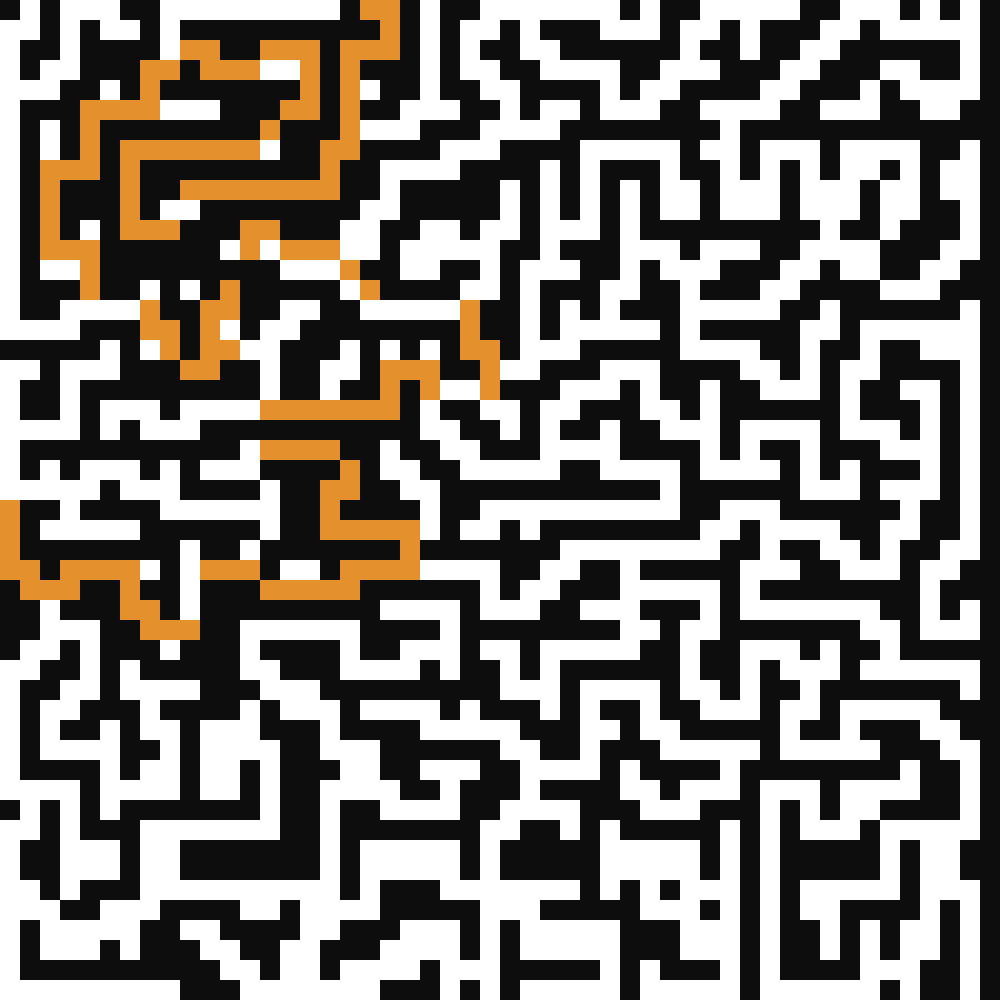
\includegraphics[width=0.62\linewidth]{figures/maze50_solution_render_hd.png}
\par\medskip
{\small\textbf{图 9.8\quad 一个 50 像素宽的已解迷宫示例}}\par
\end{minipage}
\end{center}

你应当能在项目里看到一个新文件 \texttt{sol.png}，样子大致如图 9.8。

现在，换个大点的迷宫试试，你会发现只要迷宫足够复杂，它仍会以死锁告终。原因在于：当某个 goroutine 找到解并保存进我们的 Solver 对象时，下一纳秒里，监听者停止监听通道，但其他一些探索者还在遍历自己的邻居、还在向同一个通道发布消息。一旦这个通道收到的消息达到容量上限，向它写入就会造成死锁——程序退出。下一节我们来修这个问题。

% SOURCE_PDF_PAGE: 168
\section{找到宝藏时发出通知}

我们有一个能用的方案，但它不稳定（flaky），原因有二：最明显的那个是技术问题——迷宫大到一定程度就会死锁；另一个更紧迫的是设计问题——我们结束程序前根本没有等待所有 goroutine！

因为迷宫只有一个解，找到宝藏之后，其他 goroutine 没有理由继续搜索。修好后者会顺便解决前者：如果 goroutine 停止探索，它们就不再发布新的待探索路径，通道就不会满，死锁也就消失了。

\subsection{追踪所有 goroutine}

\texttt{listenToBranches} 方法负责监听通信通道并启动 goroutine，它最清楚自己启动了多少个 goroutine、还有多少在跑。这个方法应当追踪 goroutine 并等待它们完成。追踪 goroutine 最简单的办法是使用 \texttt{sync.WaitGroup}。

给 \texttt{listenToBranches} 函数加一个等待组。每收到一条消息，先给等待组加一个追踪项，再启动新 goroutine。那个 goroutine 应当在工作完成时告知等待组。我们不想用这些逻辑污染 \texttt{explore} 方法，也不想把它散落在多个函数里，所以可以用匿名函数把 \texttt{explore} 和 \texttt{Done} 一起调用。

% SOURCE_PDF_PAGE: 169
\begin{gocode}[title={代码清单 9.25 \texttt{explore.go}：停止监听新消息}]
func (s *Solver) listenToBranches() {
    wg := sync.WaitGroup{}
    defer wg.Wait() #1
    for p := range s.pathsToExplore {
        wg.Add(1) #2
        go func(path *path) {
            defer wg.Done() #3
            s.explore(path)
        }(p) #4
        if s.solution != nil {
            return
        }
    }
}

#1 Don't leave until all goroutines are finished.
#2 Tracks one more goroutine and starts it
#3 Uses defer to make sure we don't finish early
#4 Protects the p variable
\end{gocode}

\begin{codeannotations}
\item 所有 goroutine 结束之前不离开
\item 多追踪一个 goroutine 并启动它
\item 用 \texttt{defer} 确保我们不提前收工
\item 保护 \texttt{p} 变量
\end{codeannotations}

这样我们就能确信：程序只会在所有 goroutine 结束后才结束。你可能纳闷，为什么我们用了带参数的匿名函数。原因既重要又有点复杂。迄今所有版本的 Go，直到 1.22，都受 for 循环处理方式的困扰：1.21 及更早版本会覆写用于迭代的变量——在我们的例子里就是指针 \texttt{p}。如果循环体里没有并发活动，这本来无妨，但这里情况不同。看看下面这段代码：

\begin{gocode}[]
for p := range s.pathsToExplore {
    wg.Add(1)
    go func() {
        defer wg.Done()
        s.explore(p)
    }()
}
\end{gocode}

在 Go 1.21 时，它等价于：

% SOURCE_PDF_PAGE: 170
\begin{gocode}[]
var p *path
for {
    p = <-s.pathsToExplore
    wg.Add(1)
    go func() {
        defer wg.Done()
        s.explore(p)
    }()
}
\end{gocode}

在 Go 1.22 之前，我们无法保证传给第一次 \texttt{explore} 调用的值就是我们最先从通道读到的值——等代码执行到 \texttt{s.explore} 时，它可能已被第二个值覆写。有两个常见而管用的技巧可以防止这个值被覆写。第一个就是我们前面展示的：把指针 \texttt{p} 作为启动 goroutine 的匿名函数的参数传进去（而不是在 goroutine 内部某处取用它），我们就能确保它不被覆写：只要 goroutine 还没启动，for 循环就无法从通道读下一条消息。

另一个常用的技巧是在循环体内手动复制迭代变量。多数情况下，副本使用的名字与迭代变量相同，看起来可能很怪：

\begin{gocode}[]
for p := range s.pathsToExplore {
    p := p
    wg.Add(1)
    go func() {
        defer wg.Done()
        // use the local p
        s.explore(p)
    }()
    ...
\end{gocode}

我们并不是简单地把 \texttt{p} 替换成它自己。这里是把 \texttt{for} 循环变量送进影子世界（shadow），再制作一份安全副本交给 goroutine。这个技巧在使用测试表时非常常见：我们通常会在调用 \texttt{t.Run()} 的函数中使用 \texttt{t.Parallel()}。

% SOURCE_PDF_PAGE: 171
多亏了对 \texttt{Wait()} 的调用，现在可以确信 \texttt{listenToBranches} 函数不会在 goroutine 还在探索时返回。我们不想让探索者走进死胡同（它们迟早会走到）。我们也不希望它们在岔路口再启动新 goroutine——那会白白耗费 CPU 和内存。如果我们能在知道宝藏已找到时客气地请它们停止探索，那就再好不过了。

\subsection{发送退出信号}

我们的 \texttt{explore} 函数里已经有一个停止探索的条件：只要解还没找到，无限 for 循环就继续探索。但我们不喜欢这个对 solution 的检查：这个字段既用来保存值，又被当作旗标。这让代码难以理解、难以重构，还引入了数据竞争。幸好，goroutine 之间沟通``活儿干完了''有个更好的办法——当然是通道！

\subsubsection*{添加退出通道：\texttt{select} 关键字}

我们来替换 \texttt{listenToBranches} 方法里对 solution 值的检查。我们将要求找到解的探索者向一个新通道发送消息。我们希望 \texttt{listenToBranches} 从那个通道读取，从而知道自己该停止启动探索 goroutine 了。然而，\texttt{listenToBranches} 函数已经在监听一个通道了——既然监听一个通道是阻塞的，它怎么能同时监听两个？

这正是 \texttt{select} 关键字在 Go 里的用武之地：它接受若干 case 语句（类似 switch），可以是``从通道读''或``向通道写''，最先就绪的那个被执行，
% SOURCE_PDF_PAGE: 172
其余跳过。如果多个 case 同时就绪，Go 会随机挑一个。

不过，多数时候我们感兴趣的并不只是从通道收到的第一条消息——我们想处理所有消息。为此可以用 for-select 组合，它让我们同时监听多个通道。它可以看作 \texttt{for msg := range myChannel} 循环的扩展——后者是我们用来永远监听一个通道的。在我们的例子里，可以把 for-range 循环换成行为相同的 for-select 循环：

\begin{gocode}[]
for {
    select {
    case p := <-s.pathsToExplore:
        wg.Add(1)
        go func(p *path) {
            defer wg.Done()
            s.explore(p)
        }(p)
    }
}
\end{gocode}

\texttt{select} 还接受一个 default 条目，主要用于无限 for 循环里除了 select 还有别的事可做的时候。

给 Solver 结构添加一个叫 \texttt{quit} 的通道，我们将用它通知 \texttt{listenToBranches}（稍后还有探索 goroutine 们）：解已找到，该停了。因为这个通道不承载任何有意义的消息，我们可以把它声明为空结构体的通道：\texttt{chan struct\{\}}。空结构体是 Go 的一项妙处：极其轻量（只占 0 字节），创建或复制都很快。创建 Solver 时需要在 \texttt{New} 函数里初始化这个通道：

\begin{gocode}[]
quit: make(chan struct{})
\end{gocode}

我们不需要带缓冲的通道，因为会在 \texttt{listenToBranches} 函数里监听它。看看它在

% SOURCE_PDF_PAGE: 173
下一个清单里派上用场。

\begin{gocode}[title={代码清单 9.26 \texttt{explore.go}：停止监听新消息}]
func (s *Solver) listenToBranches() {
    wg := sync.WaitGroup{}
    defer wg.Wait()
    for {
        select {
        case <-s.quit: #1
            log.Println("the treasure has been found, stopping worker")
            return
        case p := <-s.pathsToExplore: #2
            wg.Add(1)
            go func(p *path) {
                defer wg.Done()
                s.explore(p)
            }(p)
        }
    }
}

#1 Has anyone found the treasure?
#2 Keep exploring
\end{gocode}

\begin{codeannotations}
\item 有人找到宝藏了吗？
\item 继续探索
\end{codeannotations}

我们在监听 quit 通道了——但得有人往这个通道里写消息它才有用。就在 \texttt{explore} 方法里、找到宝藏的那一刻来做这件事吧。

\begin{gocode}[title={代码清单 9.27 \texttt{explore.go}：通知解已找到}]
func (s *Solver) explore(pathToBranch *path) {
    ...
    switch s.maze.RGBAAt(n.X, n.Y) {
    case s.palette.treasure:
        s.mutex.Lock()
        defer s.mutex.Unlock()
        if s.solution == nil {
            s.solution = &path{previousStep: pathToBranch, at: n}
            log.Printf("Treasure found at %v!", n)
            s.quit <- struct{}{} #1
        }
    return
}

#1 Sends a message to notify that the treasure was found
\end{gocode}

\begin{codeannotations}
\item 发送消息通知宝藏被找到
\end{codeannotations}

在几个迷宫上跑一跑，看看是否好使。因为我们用的是 goroutine，没有什么是绝对确定的，但
% SOURCE_PDF_PAGE: 174
我们这边跑它时确实出过错。监听新路径的 goroutine 一退出，仍有一些 goroutine 试图向那个通道写入——这是个阻塞动作。我们的一些探索者会陷入死锁模式，对着一个没人读的通道试图写入。到目前为止，我们只是换了个姿势到达同一个问题，但希望还在。

要解决这个问题，必须确保解一找到，探索者立刻停止探索。我们可以从 quit 通道读，但有个小难题：这一刻我们不知道还有多少探索者在跑。要让每个探索者在找到宝藏时都退出，每个探索者 goroutine 都得收到一条消息。这意味着我们要在 quit 通道里广播可能数量巨大的消息，才能保证每个探索者都收到属于自己的那条。

但有个更有意思的解法。我们可以 close 这个 quit 通道。已关闭的通道仍可读，但不可写。通道关闭后不能重新打开——这是不可撤销的最终动作。有趣之处在于：从已关闭的通道读取永远可行，而且总会返回一个值——要么是先前写入其中的值，要么，如果已没有写入值可读，就是该通道消息类型的零值。

要分辨从通道读到的值究竟是当初写进去的，还是因为我们读的是已关闭通道而被``客气地''退回的，可以用 \texttt{<-} 运算符返回的第二个值：

\begin{gocode}[]
msg, ok := <- myChannel
\end{gocode}

对我们的事来说，空结构体从哪儿来并不重要，因为我们只想尝试从 quit 通道读。
% SOURCE_PDF_PAGE: 175
只要保证没有任何东西向它写入，我们能从中读到的唯一时刻就是它被关闭之时。而且多个 goroutine 可以读一个已关闭的通道而不互相``偷走''消息，这意味着多个 goroutine 现在都能知道是不是该收工了。

把 \texttt{s.quit <- struct\{\}\{\}} 这一行换成 \texttt{close(s.quit)}。这不会改变 \texttt{listenToBranches} 方法里的代码。现在，要弄清楚在探索时如何最好地利用这个 quit 通道。

\subsubsection*{让探索者停下来}

\texttt{explore} 方法执行两项任务：在迷宫中前进，以及向监听者通报它不探索的路径。解一旦找到，这两项任务都该终止。

先想想解找到之后 \texttt{pathsToExplore} 通道会发生什么。当某个探索 goroutine 关闭 quit 通道后，\texttt{listenToBranches} 函数返回，这意味着不再有任何东西监听 \texttt{pathsToExplore} 通道——也就是说，解找到后我们就不能再向那个通道写了。怎样才能确保只在允许时才写？

不能先检查 quit 再写 \texttt{pathsToExplore}，因为那会留下一道细缝，期间另一个探索者可能恰好关闭 quit：

\begin{gocode}[]
select {
case <-s.quit:
    log.Printf("I'm an unlucky branch, someone else found the treasure, I
give up at position %v.", pos)
    return
default:
    //A goroutine could close quit between the line above and the line below
    s.pathsToExplore <- branch
}
\end{gocode}

% SOURCE_PDF_PAGE: 176
因为那道缝隙，这个方案不够安全。我们想要的是与 \texttt{listenToBranches} 方法里相同的逻辑：

\begin{gocode}[]
select {
case <-s.quit:
    log.Printf("I'm an unlucky branch, someone else found the treasure, I
give up at position %v.", pos)
    return
case s.pathsToExplore <- branch:
    //continue execution after the select block
}
\end{gocode}

在这段代码里，我们先检查 quit 是否已关闭（这是能从中读到消息的唯一情形）。如果 quit 已关闭，我们返回；否则，发布新分支。

需要注意，Go 的 select 语句对顺序不敏感（不同于 switch 语句——它从第一个选项到最后一个按优先级排）。也就是说，select 的 case 语句的顺序不决定谁先被选中。相反，如果多个 case 同时就绪，Go 会随机挑一个。在我们的例子里，select 块确保我们要么探测到 quit 信号并停止探索，要么把新分支发送到 \texttt{pathsToExplore} 通道，让程序得以继续处理其他候选，如下一个清单所示。select 语句高效地处理这些情形，不会偏爱谁。

% SOURCE_PDF_PAGE: 177
\begin{gocode}[title={代码清单 9.28 \texttt{explore.go}：仅当宝藏未找到时才探索}]
func (s *Solver) explore(pathToBranch *path) {
    // ...
    for _, candidate := range candidates[1:] {
        branch := &path{previousStep: pathToBranch, at: candidate}
        select {
        // s.quit returns a zero value only when the channel was closed
        case <-s.quit:
            log.Printf("I'm an unlucky branch, someone else found the treasure, I gi
ve up at position %v.", pos)
            return
        case s.pathsToExplore <- branch:
            // continue execution after the select block
        }
    }
\end{gocode}

最后，我们想在解找到时让探索的 goroutine 停下来。这可以做成 \texttt{explore} 方法里无限循环的第一个操作。

\begin{gocode}[title={代码清单 9.29 \texttt{explore.go}：首先，检查解是否已找到}]
func (s *Solver) explore(pathToBranch *path) {
    for {
        // Let's first check whether we should quit.
        select {
        case <-s.quit:
            return #1
        default:
            // Continue the exploration.
        }
\end{gocode}

\begin{codeannotations}
\item 停止这个探索 goroutine
\end{codeannotations}

专门用一个通道来传达``一切都该停止''是个常见模式。完整方法请看本书仓库的 \texttt{5\_notify\_treasure\_found/5\_2\_send\_quit\_signal/explore.go}（\url{https://mng.bz/KGpj}）。

现在你拥有了一个能跑的迷宫探索器，还带着几个已知的局限。如果你想扩展它，我们这里有些点子。

% SOURCE_PDF_PAGE: 178
\section{可视化}

这个口袋项目还有很多可以走得更远的地方。我们尚未提出的问题之一是含环的迷宫。设想一个迷宫含有如图 9.9 所示的局部。

\begin{center}
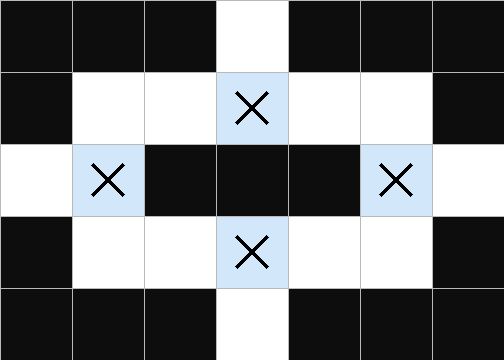
\includegraphics[width=0.36\textwidth]{figures/fig99_grid.png}

\medskip
\noindent\textbf{图 9.9\quad 带柱子的迷宫示例}
\end{center}

标着 X 的四个格位是路，但它们都绕着一个``柱子''——一块不与任何其他墙相连的墙——打转。在每个路口，goroutine 要么贴着柱子转，要么离开这个房间，但仍会制造出一个绕房间探索的分支。这意味着这样一个房间会制造出数不清的 goroutine，这对我们的计算机非常有害。我们可以要求用户提供无环迷宫，但也可以试着把这事当作探索的一部分来处理。

最后，我们确实解出了迷宫，但如果还能展示中间步骤岂不更好？这里，我们要把穿越迷宫的过程做成动画，产出一张漂亮的探索过程 GIF 文件。

% SOURCE_PDF_PAGE: 179
\subsection{克服环约束}

本章开头我们给自己立了规矩：迷宫绝不能有环。如果把它看成图，它就是一棵树——每个节点只有一条路径通向它。

如果去掉这条约束，通向宝藏的路径就可能有很多条。本章的目标并不是找最短路径。要找最短路，就得通过赋权值追踪每个像素到入口的距离，这可以用 RGBA 像素值的递增来实现。本节我们想尝试的只是找出其中一个解，并避免多次穿过相同的像素。

\subsubsection*{策略}

因为我们不想让任何 goroutine 探索之前已被探索过的像素——无论是它自己还是别的 goroutine 探索过的——我们要把这些像素当作正在探索像素的非候选邻居。为此，一个简单的技巧是：探索到它们时就把它们标记为已探索。先在 palette 结构里定义一个 explored 值：

\begin{gocode}[]
type palette struct {
    ...
    solution    color.RGBA
    explored    color.RGBA
}
\end{gocode}

接着，让 \texttt{defaultPalette} 函数为这个字段返回一个值（不同于 \texttt{palette.path} 的值）。然后，在 \texttt{explore} 函数里，我们要做的就是把正在探索的像素涂色，瞧，成了！

% SOURCE_PDF_PAGE: 180
\begin{gocode}[title={代码清单 9.30 \texttt{explore.go}：停止探索一条路径}]
func (s *Solver) explore(pathToBranch *path) {
    if pathToBranch == nil {
        // This is a safety net. It shouldn't be used,
        // but when it's needed, at least it's there.
        return
    }
    pos := pathToBranch.at
    for {
        s.maze.Set(pos.X, pos.Y, s.palette.explored) #1
        select {
\end{gocode}

\begin{codeannotations}
\item 把当前像素涂成已探索
\end{codeannotations}

\begin{center}
\begin{minipage}{0.52\textwidth}
  \centering
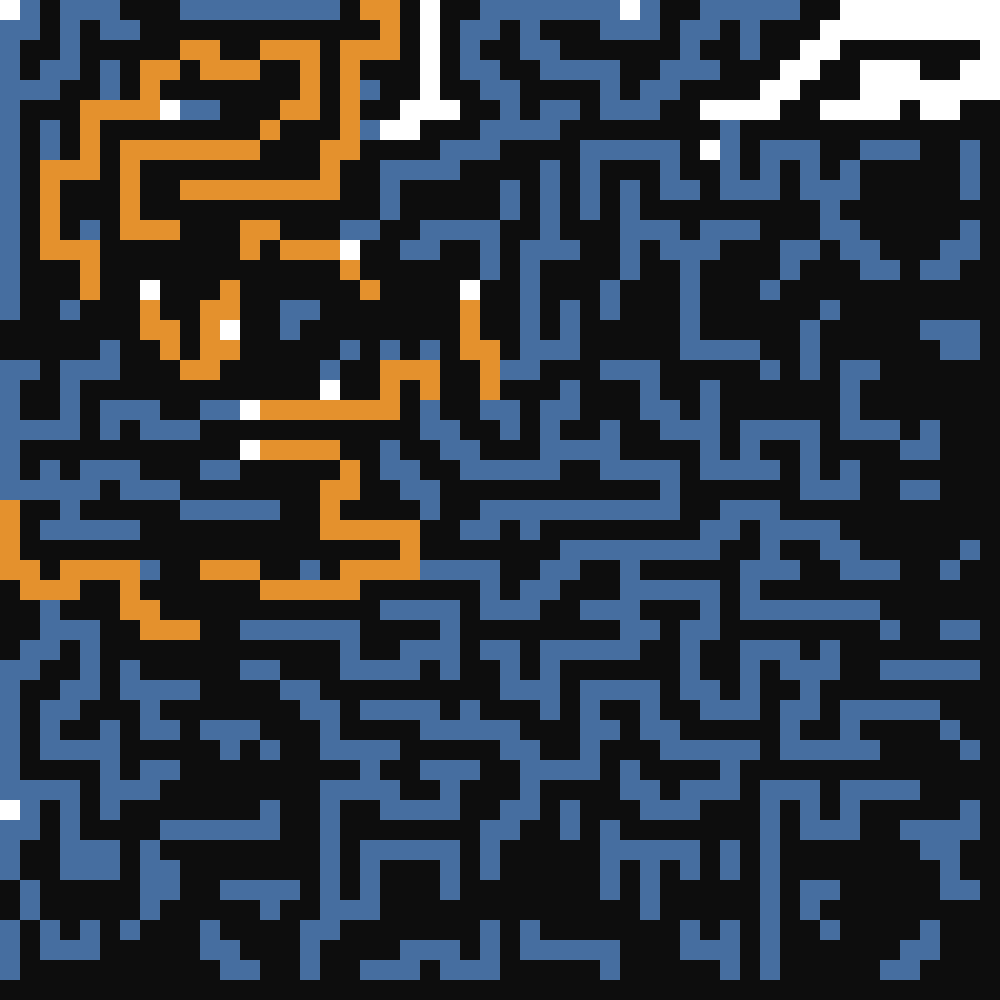
\includegraphics[width=0.78\linewidth]{figures/maze50_solved_render_hd.png}
\par\medskip
{\small\textbf{图 9.10\quad 解出的迷宫示例，已探索像素着色}}\par
\end{minipage}
\end{center}

从现在起，已探索的像素不会再成为候选——因为它不再是 \texttt{s.palette.path} 的颜色。现在运行程序，你应当会看到一幅解和已探索路径都着了色的图像，如图 9.10 所示。

\subsubsection*{实现陷阱}

且慢——我们有好几个 goroutine，而我们要每一个都去修改图像中某个像素的内容——这是数据竞争大开方便之门。在这个场景里这是个问题吗？有人可以辩称：在这种情形下这不是问题，因为无论哪个 goroutine
% SOURCE_PDF_PAGE: 181
抢先到场，结果都一样——每个 goroutine 会在那个像素写入相同的内容。任何被覆写或部分写入的值我们都能接受。但这完全错了。

\begin{infobox}{定义}
竞争条件（race condition）指的是未定义行为。不惜一切代价避免它。
\end{infobox}

根本不存在``良性竞争条件''这种东西。即便在刚才提到的情形里，同样的结果也不会出现，因为未定义行为意味着内存可能在别处被破坏，或者代码可能意外触发一颗炸弹。我们不知道。它是未定义的。编译器在把我们的代码翻译成机器语言时做了许多假设，其中之一就是：不存在数据竞争。

\subsection{让探索动起来}

我们知道自己的解能抵达宝藏。也有日志告诉我们找到了哪些死胡同。但这太不直观了，既然这是一章关于图像的内容，不如把它变得好玩些！

本节的目标是在我们穿越迷宫的过程中生成一列帧。每帧应展示给定时刻的探索状态。为此我们将用另一种图像格式——图形交换格式（GIF）——它可以用于动画（尽管这并非它最初的设计）。暂且不争论这个格式名字怎么念（至少在这章的有声书版出来之前），值得了解的是：一个 GIF 可以包含不止一个光栅帧。我们可以在单个 GIF 文件里编码多个帧，并且可以为每帧指定展示时长。这些时长
% SOURCE_PDF_PAGE: 182
以百分之一秒为单位，这是最接近屏幕刷新率的单位。既然决定要展示探索状态，该怎么做？

\subsubsection*{向 GIF 添加帧}

好，首先，我们需要能追踪到目前为止探索过的像素，这正是我们在 9.6.1 节所做的。其次，我们需要在探索的特定时刻添加帧——也就是带着当前已探索像素的图像。先给 Solver 结构加一个新字段，用标准库 \texttt{image/gif} 里的类型来持有 GIF：

\begin{gocode}[]
type Solver struct {
    ...
    animation      *gif.GIF
}
\end{gocode}

我们想什么时候给探索拍快照？如果用时间单位回答——比如每毫秒一帧——那么输出会随程序在不同电脑上跑得快慢而不同。否则，也可以考虑每发现 10 个新像素就展示一次状态。这虽然可行，但迷宫一大问题就严重了。假设迷宫含 40\% 的路径像素：在 10×10 的迷宫里约有 40 个路径像素可探索——那会做出一个 4 帧的 GIF。可是在 1000×1000 的迷宫里，约有 400000 个像素要探索，得到一个 40000 帧的 GIF。这样的文件一来非常重，二来如果每帧给百分之一秒的展示时间，最坏情况下要超过 6 分钟才能把探索放完。

% SOURCE_PDF_PAGE: 183
换个思路：我们干脆规定，如果探索整座迷宫，最终的 GIF 就要 30 帧长。这是个人为定的数，但做出来的动画不会太长。这意味着每探索 (总可探索像素)/(30 像素) 个像素，就要打印一次探索状态。我们需要为动画统计所有可探索像素，那就在新文件 \texttt{animation.go} 里写个函数吧。

\begin{gocode}[title={代码清单 9.31 \texttt{animation.go}：统计所有可探索像素}]
// countExplorablePixels scans the maze and counts the number
// of pixels that are not walls.
func (s *Solver) countExplorablePixels() int {
    explorablePixels := 0
    for row := 0; row < s.maze.Bounds().Dy(); row++ { #1
        for col := 0; col < s.maze.Bounds().Dx(); col++ { #2
            if s.maze.RGBAAt(col, row) != s.palette.wall { #3
                explorablePixels++
            }
        }
    }
    return explorablePixels
}

#1 The outer loop is on rows.
#2 The inner loop is on columns.
#3 Count path + treasure + entrance
\end{gocode}

\begin{codeannotations}
\item 外层循环在行上
\item 内层循环在列上
\item 统计路径 + 宝藏 + 入口
\end{codeannotations}

在 9.6.1 节里，我们遇到新的未探索像素时增加了一个操作——把它涂色。这里，我们想遇到新像素时再干点别的事。这需要把这些动作重构为 Solver 结构上的一个方法，不妨叫 \texttt{registerExploredPixel}。这个函数会把已探索像素涂色，并且根据已探索的数量，把帧添加进动画。然而，给像素涂色花不了多久，把帧添加进动画却意味着复制整幅图像，可能耗时很长。我们不想让这种复制阻塞任何探索进程，这意味着要让探索者异步地发送``有新像素待注册''的通知。

% SOURCE_PDF_PAGE: 184
Go 里做异步调用主要有两种方式。第一种是放进 goroutine 里调用：

\begin{gocode}[]
go s.registerExploredPixel(pos)
\end{gocode}

这完全可行，但我们必须自问：会不会发生竞争条件？归根结底，这个方法将需要显式使用互斥锁。但关于 goroutine 之间的通信我们说过什么来着？答案引出第二种做法，也是我们在此要用的：用一个通道，探索者把想注册的像素发送进去。这样一来，\texttt{registerExploredPixel} 从通道接收像素。只要我们逐一处理从通道读出的像素，就不需要互斥锁。把这个通道加进 Solver 结构吧。别忘了在 \texttt{New} 函数里初始化它：

\begin{gocode}[]
type Solver struct {
    ...
    exploredPixels chan image.Point
    animation      *gif.GIF
}
\end{gocode}

探索者的无限 for 循环可以更新为：要么在 quit 通道因找到解而关闭时中止，要么发送一个像素去注册并继续探索，如下面的清单所示。

% SOURCE_PDF_PAGE: 185
\begin{gocode}[title={代码清单 9.32 \texttt{explore.go}：把像素注册为已探索}]
func (s *Solver) explore(pathToBranch *path) { #1
    ...
    for {
        // Let's first check whether we should quit.
        select {
        case <-s.quit:
            return
        case s.exploredPixels <- pos: #1
            // Continue the exploration.
        }
    }
    ...
}

#1 Replaces the previous default case
\end{gocode}

\begin{codeannotations}
\item 替换先前的 default 分支
\end{codeannotations}

现在可以编写负责注册已探索像素的函数了，如代码清单 9.33 所示。要知道该多久写一帧，我们定义 \texttt{totalExpected­Frames} 为输出 GIF 想要的帧数——比方说最多 30 帧。我们不会精确得到 30 帧，因为我们不会探索每个像素。接着统计可探索像素的总数，然后用 for-select 模式持续运行，直到被告知退出。

每收到一个新探索像素的位置，我们就把它涂色、给已探索计数器加一，并在达到阈值时画一帧。

% SOURCE_PDF_PAGE: 186
\begin{gocode}[title={代码清单 9.33 \texttt{animation.go}：实现 \texttt{registerExploredPixels}}]
// registerExploredPixels registers positions as explored on the image,
// and, if we reach a threshold, adds the frame to the output GIF.
func (s *Solver) registerExploredPixels() {
    const totalExpectedFrames = 30
    explorablePixels := s.countExplorablePixels() #1
    pixelsExplored := 0
    for {
        select {
        case <-s.quit: #2
            return
        case pos := <-s.exploredPixels: #3
            s.maze.Set(pos.X, pos.Y, s.palette.explored) #4
            pixelsExplored++
            if pixelsExplored%(explorablePixels/totalExpectedFrames) == 0 {
                s.drawCurrentFrameToGIF()
            }
        }
    }
}

#1 Checks how many pixels are explorable
#2 Checks whether we should quit first
#3 Reads positions that have been explored
#4 Paints explored pixels
\end{gocode}

\begin{codeannotations}
\item 检查有多少像素可探索
\item 先检查是否应当退出
\item 读取已探索的位置
\item 把已探索像素涂色
\end{codeannotations}

现在来讨论 \texttt{drawCurrentFrameToGIF} 方法：它做什么、我们怎么画帧。首先，看看 \texttt{go doc gif.GIF.Image} 就会发现，GIF 结构使用的是调色板图像（paletted image）切片。这是一种压缩算法：图像用到的每种颜色存进一个调色板，每个像素不再用经典的 RGBA 值编码，而是用它颜色在调色板中的键编码。调色板的颜色数通常远少于整个 RGBA 光谱能提供的，这有时会导致结果图像出现压缩伪影。

创建调色板图像相当直接，因为 Go 有一个 \texttt{image/color/palette} 包，它只提供两个调色板——Plan9 和 WebSafe（还贴心地提到``早期版本的 Netscape Navigator''）。这里的选择权在你。我们还得决定：GIF 动画是与初始迷宫同尺寸，还是固定尺寸。与输入图像同尺寸更简单，但会让
% SOURCE_PDF_PAGE: 187
大多数 GIF 过小或过大。让帧与迷宫尺寸不同就需要像素插值，稍后几行就会看到。为了本章的目的，我们给每帧取固定宽度 500 像素、高度按输入图像像素的相同比例：

\begin{gocode}[]
const gifSize = 500
frame := image.NewPaletted(image.Rect(0, 0, gifSize, gifSize*s.maze.Bounds().Dy()/s.
maze.Bounds().Dx()), palette.Plan9)
\end{gocode}

在代码里使用 \texttt{image/color/palette} 会引起冲突！我们包里已经有一个叫 \texttt{palette} 的类型，它定义墙和路应当是什么颜色。通过给导入起别名，我们可以轻松化解这个冲突。

\begin{infobox}{注意}
在 Go 里，给导入起别名有时很有用。这里我们会用 \texttt{import plt "image/color/palette"}。给导入起别名时，最好用与原包名相似的别名，以保持代码清晰。
\end{infobox}

我们创建了一块空画布，下面把已探索迷宫的当前状态画上去。遗憾的是，Go 的 \texttt{image/draw} 包不支持缩放图像，因此也不支持任何插值。我们得用 \texttt{golang.org/x/image/draw}——它的功能更全的版本。这个包提供了 \texttt{golang.org/x/image/draw.Scaler} 接口，可以把输入图像的一个矩形区域缩放为输出图像的一个矩形区域。\texttt{golang.org/x/image/draw} 暴露了三个实现 Scaler 接口的类型：\texttt{Nearest­Neighbor}、\texttt{CatmullRom} 和 \texttt{ApproxBiLinear}。出于本章的目的，我们坚持用 \texttt{NearestNeighbor}，因为它不会把像素边缘弄糊：

\begin{gocode}[]
draw.NearestNeighbor.Scale(frame, frame.Rect, s.maze, s.maze.Bounds(),
draw.Over, nil)
\end{gocode}

% SOURCE_PDF_PAGE: 188
最后，把帧添加进我们的 GIF 图像。这三项操作可以写进一个由 \texttt{markPixelExplored} 调用的方法。

\begin{gocode}[title={代码清单 9.34 \texttt{animation.go}：把帧画到 GIF 上}]
package solver

import (
    "image"
    plt "image/color/palette" #1
    "golang.org/x/image/draw"
)

// ...
// drawCurrentFrameToGIF adds the current state of the maze
// as a frame of the animation.
func (s *Solver) drawCurrentFrameToGIF() {
    const (
        // gifWidth is the width of the generated GIF.
        gifWidth = 500
        // frameDuration is the duration in hundredth of a second
        // of each frame.
        // 20 hundredths of a second per frame means 5 frames per second.
        frameDuration = 20
    )
    // Create a paletted frame that has the same ratio as the input image
    frame := image.NewPaletted(image.Rect(0, 0, gifSize,
        gifWidth*s.maze.Bounds().Dy()/s.maze.Bounds().Dx()), plt.Plan9)
    // Convert RGBA to paletted
    draw.NearestNeighbor.Scale(
        frame, frame.Rect, s.maze, s.maze.Bounds(), draw.Over, nil)
    s.animation.Image = append(s.animation.Image, frame)
    s.animation.Delay = append(s.animation.Delay, frameDuration)
}

#1 Aliases the import to avoid conflict with the type palette
\end{gocode}

\begin{codeannotations}
\item 给导入起别名，避免与类型 \texttt{palette} 冲突
\end{codeannotations}

现在我们有了一个单独的 goroutine 负责更新图像像素的值，它随着像素从通道到来而逐个处理。别忘了在 Solve 里启动这个 \texttt{registerExploredPixels} 方法。现在我们有两个想启动的``监听'' goroutine——\texttt{listenToBranches} 和 \texttt{registerExploredPixels}。要把两者都启动、并在它们返回后同步，可以用 \texttt{sync.WaitGroup}。

% SOURCE_PDF_PAGE: 189
\begin{gocode}[title={代码清单 9.35 \texttt{solver.go}：在 \texttt{Solve} 里启动监听者}]
func (s *Solver) Solve() error {
    // ...
    log.Printf("starting at %v", entrance)
    s.pathsToExplore <- &path{previousStep: nil, at: entrance}
    wg := sync.WaitGroup{}
    wg.Add(2)
    defer wg.Wait() #1
    go func() { #2
        defer wg.Done()
        // Launch the goroutine in charge of drawing the GIF image.
        s.registerExploredPixels()
    }()
    go func() { #3
        defer wg.Done()
        // Listen for new paths to explore.
        // This only returns when the maze is solved.
        s.listenToBranches()
    }()
    return nil
}

#1 Solve won't return unless both goroutines are done.
#2 One goroutine to register explored pixels
#3 One goroutine to explore new branches
\end{gocode}

\begin{codeannotations}
\item 两个 goroutine 不都完成，\texttt{Solve} 就不返回
\item 一个 goroutine 注册已探索像素
\item 一个 goroutine 探索新分支
\end{codeannotations}

\subsubsection*{生成 GIF 文件}

现在我们已经把帧加进了 GIF。每帧都是从正在探索的迷宫逐像素复制来的。

接下来，把 GIF 文件画出来。为此，只需在代码里知道``可以打印了''的位置接上一个写出动画输出图像的函数调用。现有的 \texttt{SaveSolution} 函数是绝佳选择，因为它已经负责写一个输出文件了。我们在那里调用一个新方法来画最终的 GIF。

% SOURCE_PDF_PAGE: 190
\begin{gocode}[title={代码清单 9.36 \texttt{imagefile.go}：生成 GIF 文件}]
func (s *Solver) SaveSolution(outputPath string) error {
     // ...
    gifPath := strings.Replace(outputPath, "png", "gif", -1)
    err = s.saveAnimation(gifPath)
    if err != nil {
        return fmt.Errorf(...)
    }
    return nil
}

// saveAnimation writes the gif file.
func (s *Solver) saveAnimation(gifPath string) error {
    outputImage, err := os.Create(gifPath)
    if err != nil {
        return fmt.Errorf(...)
    }
    defer func() {
        if closeErr := outputImage.Close(); closeErr != nil {
            // Return err and closeErr, in worst case scenario.
            err = errors.Join(err,
                fmt.Errorf("unable to close file: %w", closeErr))
        }
    }()
    log.Printf("animation contains %d frames\n", len(s.animation.Image))
    err = gif.EncodeAll(outputImage, s.animation)
    if err != nil {
        return fmt.Errorf("unable to encode gif: %w", err)
    }
    return nil
}
\end{gocode}

这段代码与 PNG 图像编码的代码非常相似。现在，让我们运行程序：

\begin{shellcode}[]
> go run . mazes/maze50_50.png solution.png
2023/10/18 11:42:57 INFO Solving maze "mazes/maze50_50.png" and saving it
as "solution.png"
2023/10/18 11:42:57 INFO starting at (0,25)
2023/10/18 11:43:00 INFO Treasure found: (18,0)!
2023/10/18 11:43:00 INFO the treasure has been found, worker going to sleep
2023/10/18 11:43:00 INFO animation contains 30 frames
\end{shellcode}

这应当会生成 \texttt{solution.png} 图像以及一个 \texttt{solution.gif} 文件。打开这个文件，看看迷宫是如何被探索的。你注意到什么了吗？解显示得并不清楚——如果它有显示的话——而且循环马上重新开始。要是能把
% SOURCE_PDF_PAGE: 191
解加进帧列表、并让这最后一帧打印得更久一些，那就好了。

在 9.4 节，我们把解的涂色加进了 \texttt{SaveSolution} 方法。现在需要对 GIF 做点事，我们也许想要一个专门的方法，把这段逻辑从写文件的代码挪到 Solver 里。让我们为本章写下最后几行代码。先把 Solver 存储的图像里入口与解之间的像素涂色，然后向 GIF 添加最后一帧（包含涂了解的像素），如下面的清单所示。通过设一个更长的值，我们确保最后一帧会展示得足够久，好让人细细欣赏。

\begin{gocode}[title={代码清单 9.37 \texttt{solver.go}：保存解，为探索收尾}]
func (s *Solver) Solve() error {
    // ...
    wg.Wait()
    s.writeLastFrame()
    return nil
}

// writeLastFrame writes the last frame of the gif,
// with the solution highlighted.
func (s *Solver) writeLastFrame() {
    stepsFromTreasure := s.solution
    // Paint the path from entrance to the treasure.
    for stepsFromTreasure != nil { #1
        s.maze.Set(stepsFromTreasure.at.X, stepsFromTreasure.at.Y,
            s.palette.solution)
        stepsFromTreasure = stepsFromTreasure.previousStep
    }
    const solutionFrameDuration = 300 // 3 seconds
    // Add the solution frame, with the coloured path, to the output gif.
    s.drawCurrentFrameToGIF()  #2
    s.animation.Delay[len(s.animation.Delay)-1] = solutionFrameDuration
}

#1 Makes sure the treasure is found
#2 Draws the final frame of the GIF with a longer duration
\end{gocode}

\begin{codeannotations}
\item 确保宝藏被找到
\item 画出 GIF 的最后一帧，并给予更长的展示时间
\end{codeannotations}

重新运行程序，打开 GIF。你可以调整帧时长或帧数，
% SOURCE_PDF_PAGE: 192
来获得你真正想要的观感。遗憾的是，我们没法把 GIF 放进书里——把你的 GIF 分享给朋友们吧！

\section*{小结}

\begin{itemize}
\item 在计算机科学中，2D 图像的主要类型是光栅图像和矢量图像。
\item 矢量图像用于字体和标志、信息图或图标。矢量图像缩放性极好——放大也看不到任何伪影。
\item 我们使用的另一半图像是光栅图像——像素组成的 2D 网格。图像的每个像素都有一种颜色，可以用 RGBA 颜色模型表示（但也可能以其他颜色模型编码，比如 JPEG 图像的 YCbCr）。颜色的值既可以用来编码物理信息，比如物体发出的红、绿、蓝频率光的强度（如一张花的照片），也可以编码任何数值信息（例如人口密度）。此外，还可以用调色板来表示同属一类的区域，比如地图上每个国家有自己的颜色。
\item \texttt{image/png} 包用于把文件 Decode 成 \texttt{image.Image}。这个 Image 经常被类型断言为 RGBA 或 NRGBA。要编码图像，请用你想把图像编码成的那个包的 Encode 函数——可选的是 gif、jpeg 和 png。其他格式需要第三方库。
\item 图像通常把 (0, 0) 位置的像素放在左上角。然而，有些图像的 (0, 0) 可能在任何一个角。这完全取决于图像格式和图像元数据。请使用 \texttt{image} 包返回的内容来迭代图像的像素。
% SOURCE_PDF_PAGE: 193
\item 可以用 \texttt{.At()} 方法访问 \texttt{image.Image} 中像素的值。它返回一个 \texttt{color.Color()}，你必须把它转换成 \texttt{color.RGBA}。使用 \texttt{image.RGBA} 时，可以改用 \texttt{RGBAAt()}，它返回的 \texttt{color.RGBA} 可直接与已知值比较。
\item 要向 \texttt{image.RGBA} 写入像素，使用 \texttt{Set(x, y, rgba)} 方法。
\item 扫描整幅图像时，使用两层嵌套循环——最外层遍历行，最内层遍历列。这对所有扫描线格式的性能都有好处。
\item 当无法使用全局常量时，用一个返回配置值的函数比用全局变量稍显干净。出于安全考虑，避免暴露全局变量：其他代码可能会改掉它们。
\item 向一个无人读取的无缓冲通道写入是阻塞的。要么在 goroutine 里写，要么使用带缓冲通道——其大小应当是读取开始之前会写入那里的元素的最大数量。
\item 在循环里启动 goroutine 时，确保循环变量受到保护。循环变量可能是你从通道读出的消息、你遍历的映射的键或值，或者切片的元素。在循环内部启动 goroutine 时，保护 for 循环迭代器有三种常见方式：
  \begin{itemize}
  \item 使用保证这一点的 Go 版本（目前，这被认为是 Go 1.22）。
  \item 在循环里用另一个变量遮蔽（shadow）循环变量（通常，我们给新变量起与循环变量相同的名字）。
  \item 用一个把循环变量作为参数的匿名函数来启动 goroutine。
  \end{itemize}
% SOURCE_PDF_PAGE: 194
\item \texttt{select} 关键字允许一段代码监听多个通道。只要任一通道发布了消息，对应 case 语句里写的代码就会被执行。
\item 如果 select 中有多个 case 语句都就绪，Go 会随机挑一个。
\item select 的某个 case 语句常常充当返回条件。在服务器里尤其如此：一旦请求被取消，对该输入请求的处理就应当尽快结束。
\item for-select 无限循环的监听模式非常常见。通常，select 块的某个 case 会包含退出循环的条件。
\end{itemize}
